\documentclass[a4paper, 11pt, oneside]{report}
\usepackage[left=1in, right=1in, top=1in, bottom=1in]{geometry}
\newcommand{\plogo}{\fbox{$\mathcal{PL}$}}
\usepackage{graphicx}
\graphicspath{{figures/}}
\usepackage{graphics}
\usepackage{float}
\usepackage[table,xcdraw]{xcolor}
\usepackage[utf8]{inputenc}
\usepackage[T1]{fontenc}
\usepackage{fouriernc}
\usepackage{subcaption}
\usepackage{tikz}
\usetikzlibrary{shapes.geometric, arrows, arrows.meta, positioning, fit, calc, backgrounds}

% ---- Shared diagram design system (one restrained visual language for all figures) ----
\tikzset{
  vgnode/.style={draw=black!72, line width=0.5pt, rounded corners=2pt, fill=black!4,
                 align=center, font=\small, inner sep=6pt, minimum height=0.9cm},
  vgacc/.style={vgnode, fill=blue!7, draw=blue!50!black},
  vgext/.style={draw=black!72, line width=0.5pt, sharp corners, fill=black!9,
                align=center, font=\small, inner sep=6pt, minimum height=0.9cm},
  vgproc/.style={draw=black!72, line width=0.5pt, circle, fill=black!4,
                 align=center, font=\footnotesize, inner sep=1pt, minimum size=1.5cm},
  % classic open (DeMarco) data store: top + bottom rule only
  vgds/.style={draw=none, fill=none, align=center, font=\footnotesize, inner sep=4pt,
               minimum width=2.5cm, minimum height=0.78cm,
               append after command={\pgfextra{%
                 \draw[black!72, line width=0.5pt] (\tikzlastnode.north west)--(\tikzlastnode.north east);
                 \draw[black!72, line width=0.5pt] (\tikzlastnode.south west)--(\tikzlastnode.south east);}}},
  vgflow/.style={-{Stealth[length=1.8mm,width=1.4mm]}, line width=0.55pt, draw=black!72, rounded corners=2.5pt},
  vgbi/.style={{Stealth[length=1.8mm,width=1.4mm]}-{Stealth[length=1.8mm,width=1.4mm]},
               line width=0.55pt, draw=black!72, rounded corners=2.5pt},
  vgdash/.style={vgflow, dashed},
  vglbl/.style={font=\footnotesize, text=black!78, inner sep=1.6pt, fill=white}
}
\usepackage{pgfplots}
\pgfplotsset{compat=1.18}
\usepackage{longtable}
\usepackage[nottoc]{tocbibind}
\usepackage{url}
\usepackage{hyperref}
\usepackage{amsmath}
\usepackage{amssymb}
\usepackage{pgfgantt} % For Gantt charts
\usepackage{pdflscape} % For landscape pages if a chart is wide
\usepackage{booktabs} % For better tables
\usepackage{multirow}
\usepackage[boxed]{algorithm}
\usepackage{algpseudocode}
\usepackage[none]{hyphenat}
\usepackage{listings}

\lstset{
  basicstyle=\ttfamily\footnotesize,
  breaklines=true,
  frame=single,
  columns=fullflexible,
  keepspaces=true,
  showstringspaces=false
}

\begin{document}
    \sloppy
    \setlength{\parindent}{0em}
    \setlength{\parskip}{0.5em}

	\begin{titlepage}

		\centering

		\vspace*{\baselineskip}

		\vspace{0.75\baselineskip}

		{\LARGE \textbf{VeriGate: An Adaptive, Self-Verifying Semantic Cache for Scalable and Cost-Efficient LLM Gateways}}

		\vspace{0.75\baselineskip}

		\vspace{2\baselineskip}

		A report submitted for the course named Project - II (CS4201)

		\vspace*{7\baselineskip}

		Submitted By

		\vspace{0.5\baselineskip}

		{\scshape\Large ABHISHEK YADAV \\ SEMESTER - VII \\ 230103041}

		\vspace{0.5\baselineskip}

		Supervised By

		\vspace{0.5\baselineskip}

		{\scshape\Large Dr. Salam Michael Singh}
		\vspace{0.5\baselineskip}

		\vfill

		\begin{center}
			
\includegraphics[width=5cm]{iiit_manipur.png}
		\end{center}

	{\scshape\small Department of Computer Science and Engineering\\ Indian Institute of Information Technology Senapati, Manipur \\ November, 2026}

\end{titlepage}

%----------------------------------------------------------------------------------------

\begin{center}
   { \LARGE \textbf{Declaration}}
\end{center}
In this submission, I have expressed my idea in my own words, and I have adequately cited and referenced any ideas or words that were taken from another source. I also declare that I adhere to all principles of academic honesty and integrity and that I have not misrepresented or falsified any ideas, data, facts, or sources in this submission. If any violation of the above is made, I understand that the institute may take disciplinary action. Such a violation may also engender disciplinary action from the sources which were not properly cited or permission not taken when needed.

\vspace{1cm}\hspace{8.35cm} ABHISHEK YADAV \\
\vspace{1cm}\hspace{9cm} 230103041 \\

\newpage

\begin{center}
	\thispagestyle{empty}

		\begin{table}
			\centering
			
\includegraphics[scale=0.2]{iiit_manipur.png}
			\begin{tabular}{l}
				Department of Computer Science and Engineering \\
				Indian Institute of Information Technology Senapati, Manipur \\
			\end{tabular}
		\end{table}
		\par\noindent\rule{\textwidth}{0.4pt}
			\textbf{Dr. Salam Michael Singh}
			\hspace*{\fill} Email: \href{mailto:michael_s@iiitmanipur.ac.in}{michael\_s@iiitmanipur.ac.in}\\
			Assistant Professor
			\hspace*{0pt}\hfill Contact No: +91 8575443081\\[2cm]
			{\Huge \textbf{\emph{To Whom It May Concern}}}\\[2cm]
			\linespread{1.13}
			\large{This is to certify that the project report
                entitled \textbf{"VeriGate: An Adaptive, Self-Verifying Semantic Cache for Scalable and Cost-Efficient LLM Gateways",} submitted to the department of Computer Science and Engineering, Indian Institute of Information Technology Senapati, Manipur in partial fulfillment for the award of degree of Bachelor of Technology in Computer Science and Engineering is a bonafide record of work carried out by \textbf{ABHISHEK YADAV} bearing roll number 230103041.}\\[2.0cm]
			\hspace*{2.6in}\large{Signature of Supervisor}\\[0.3cm]
			\hspace*{2.5in}\textbf{(Dr. Salam Michael Singh)}\\[0.5cm]

	\end{center}
        \vspace{0.5cm}
	Signature of the Examiner 1 ............................\\\\
	Signature of the Examiner 2 ............................\\\\
	Signature of the Examiner 3 ............................\\\\
	Signature of the Examiner 4 ............................\\\\
	\newpage


\newpage
\addcontentsline{toc}{chapter}{Abstract}
\begin{center}
    { \LARGE \textbf{Abstract}}
\end{center}
\vspace{1.5cm}
{\large
Large Language Models (LLMs) are increasingly deployed in production, but every API call incurs monetary cost and high latency. A \textit{semantic cache} mitigates this by returning a stored answer when a new query is semantically ``close enough'' to a past one. However, existing semantic caches (e.g. GPTCache) rely on a \textbf{single fixed similarity threshold}, which produces \textbf{false cache hits} --- serving the wrong stored answer to a look-alike query (for example, returning the answer for \textit{``capital of Austria''} to \textit{``capital of Australia''}). This report presents \textbf{VeriGate}, a production-grade LLM Gateway whose core novel contribution is an \textbf{adaptive, self-verifying semantic cache}: it (i) adapts the similarity threshold per query using neighbourhood density, (ii) \textit{verifies} a candidate hit with a two-tier verifier (a near-free structural check on numbers, negation and named entities, and an optional NLI cross-encoder), and (iii) detects volatile queries to skip caching time-sensitive answers. A second contribution, a \textbf{cost-aware model cascade}, routes easy queries to a cheap model and escalates only hard ones. On a controlled benchmark, VeriGate reduces the false-hit rate from the fixed-threshold baseline's \textbf{46.7\%} to \textbf{0.0\%} (100\% precision), with structural verification costing only \textbf{$\sim$0.03~ms}; a vectorised index brings the cache-hit path to \textbf{$\sim$10~ms} ($\sim$78$\times$ faster than an 800~ms LLM call), and the cascade cuts LLM cost by \textbf{$\sim$47\%} with no quality loss on hard queries. The system is engineered for production with per-tenant cache isolation, per-key spend budgets, a provider circuit breaker, Prometheus/Grafana observability, and Docker packaging.
}

\newpage
        \begin{center}
            { \LARGE \textbf{Acknowledgement}}
        \end{center}
	\vspace{2cm}
	I would like to express my deepest appreciation to all those who provided me the possibility to complete this project. A special gratitude I give to my supervisor, \textbf{Dr. Salam Michael Singh}, whose contribution in stimulating suggestions and encouragement helped me to coordinate my project especially in writing this report.

	I would also like to express my sincere gratitude to the Head of the Department (CSE), \textbf{Dr. Navanth Saharia}, for his constant support and for providing the necessary facilities to successfully execute this project.

	Furthermore, I would also like to acknowledge with much appreciation the crucial role of the faculty and staff of the Department of Computer Science and Engineering, Indian Institute of Information Technology Senapati, Manipur, who gave the permission to use all required equipment and necessary materials to complete the tasks.

	Last but not least, many thanks go to my family and friends whose support, guidance, and encouragement have been invaluable throughout this endeavor.

	\vspace{1cm}
	\begin{flushright}
	    \textbf{ABHISHEK YADAV} \\
	    Roll No: 230103041
	\end{flushright}

	\vspace{1cm}

	\addcontentsline{toc}{chapter}{Acknowledgement}
	\tableofcontents
	\listoffigures
        \listoftables
	\chapter{Introduction}
	\section{Background}
Large Language Models (LLMs) such as the GPT and Gemini families have moved rapidly from research artifacts into production software, powering chat assistants, retrieval-augmented question answering, code generation, and agentic workflows. The transformer architecture that underpins them \cite{vaswani2017attention, devlin2019bert} delivers remarkable general-purpose language capability, but it does so at a recurring price: every request to a hosted LLM incurs a per-token monetary cost and a network-and-inference latency that is frequently measured in seconds rather than milliseconds. At the scale of a real application serving thousands of users, these two quantities --- cost and latency --- become the dominant operational constraints, and reducing them without degrading answer quality is a central problem in efficient LLM serving \cite{zhu2023survey}.

A widely adopted mitigation is the \textbf{semantic cache}. A conventional cache keys on an exact string, so it only helps when the identical request repeats. A semantic cache instead embeds the incoming query into a dense vector \cite{reimers2019sentencebert} and, if a previously answered query lies ``close enough'' in that vector space, returns the stored answer without calling the LLM at all. Because natural-language questions are frequently reworded (\textit{``how do I reset my password''} versus \textit{``what is the process to recover my account password''}), a semantic cache captures far more reuse than an exact cache, converting a slow, paid model call into an instant, free lookup. Open-source systems such as GPTCache \cite{bang2023gptcache} have popularised this pattern.

However, the semantic cache carries a failure mode that the exact cache does not. Because it serves an answer whenever similarity crosses a threshold, two questions that are lexically and semantically \emph{close} but factually \emph{distinct} can collide. The canonical example is \textit{``what is the capital of Austria''} versus \textit{``what is the capital of Australia''}: the two sentences differ by two characters, embed very near each other, and yet demand entirely different answers. When a fixed-threshold cache serves the stored ``Vienna'' answer to the ``Australia'' query, it commits a \textbf{false cache hit} --- confidently returning a wrong answer. This is more dangerous than a cache \emph{miss}, because a miss merely forfeits a saving whereas a false hit silently corrupts correctness.

\section{Motivation}
The motivation for this project is the observation that the quality of a semantic cache is governed almost entirely by a single, brittle hyper-parameter: the similarity threshold. Set it too high and the cache rarely fires, forfeiting the cost and latency savings that justify its existence. Set it too low and false hits proliferate. Crucially, \emph{no single fixed threshold is correct for all queries.} The ideal threshold depends on how densely the neighbourhood around a query is populated, on how factually load-bearing the query's tokens are (a swapped digit or a negation flips the answer), and on whether the query is even cacheable at all (a request for \textit{today's} weather must never be served from yesterday's cache).

Existing systems treat this as a configuration value the operator must guess, and they trust the similarity score alone to decide a hit. There is therefore a clear gap between the \emph{detection} of a nearby cached answer and the \emph{verification} that the answer is actually correct for the new question. Bridging that gap --- making the cache adapt its strictness per query and \emph{verify} a candidate hit before serving it --- is the intellectual core of this work. A cache that can decline to answer when it is not sure, rather than confidently serving a look-alike, represents a safer and more deployable design.

A second, complementary motivation is cost. Even with a perfect cache, the queries that \emph{do} reach the LLM need not all go to the most expensive model. Many are trivial and can be answered correctly by a small, cheap model; only the genuinely hard queries warrant an expensive one. A gateway that routes by query difficulty can cut spend substantially without sacrificing quality on the queries that matter.

\section{Problem Definition}
The core problem addressed in this project is that contemporary semantic caches for LLMs are \textbf{fixed-threshold and unverified}, which makes them unsafe: they trade correctness for savings in a way the operator cannot tune away. Specifically, the problem decomposes into the following sub-challenges:

\begin{enumerate}
    \item \textbf{Threshold brittleness.} A single global similarity threshold cannot simultaneously maximise reuse and avoid false hits, because the correct strictness is query-dependent. The optimal threshold also shifts with the embedding model, so a value tuned for one embedder is wrong for another.
    \item \textbf{Unverified hits (the false-hit problem).} Similarity above a threshold is not proof of semantic equivalence. Queries differing only in a number, a negation, or a named entity embed very close together yet require different answers, and a naive cache serves the wrong one.
    \item \textbf{Uncacheable (volatile) queries.} Time-sensitive queries (\textit{``weather today''}, \textit{``current stock price''}) must never be served from cache, but a similarity-only cache has no notion of staleness.
    \item \textbf{Latency of the cache itself.} A cache is only worthwhile if the lookup is dramatically faster than the LLM call it replaces; a naive linear scan over stored vectors degrades as the cache grows.
    \item \textbf{Uniform-cost routing.} Sending every cache-missed query to a single expensive model wastes money on queries a cheap model would answer correctly.
    \item \textbf{Production safety.} A shared cache in front of an LLM introduces multi-tenant data-leakage, cost-exhaustion, and reliability risks that a research prototype typically ignores.
\end{enumerate}

\section{Project Objectives}
To address the above, this project designs, implements, and evaluates \textbf{VeriGate}, a production-grade LLM Gateway. The main objectives are:

\begin{itemize}
    \item \textbf{Adaptive similarity threshold.} To raise or lower the effective threshold \emph{per query} based on the density of the query's neighbourhood in embedding space, so that ambiguous regions are treated more strictly than isolated ones (Section~\ref{sec:adaptive}).
    \item \textbf{A self-verifying cache (the central contribution).} To interpose a two-tier verifier between a candidate hit and the served answer: a near-free Tier-1 structural check on numbers, negation, and named entities, and an optional Tier-2 Natural Language Inference (NLI) check for bidirectional entailment, so that a look-alike whose similarity is \emph{above} the threshold is still rejected (Section~\ref{sec:verifier}).
    \item \textbf{Volatility detection.} To classify time-sensitive queries and bypass the cache for them, preventing stale answers (Section~\ref{sec:volatility}).
    \item \textbf{A sub-linear cache-hit path.} To replace the naive linear scan with a vectorised in-process index (and an optional distributed RediSearch/HNSW backend \cite{malkov2018hnsw, redis_stack}) so that the hit path stays an order of magnitude faster than an LLM call as the cache scales (Section~\ref{sec:index}).
    \item \textbf{A cost-aware model cascade (second contribution).} To score query complexity and route easy queries to a cheap model, escalating only hard ones to a strong model, cutting cost while preserving quality on hard queries \cite{chen2023frugalgpt} (Section~\ref{sec:cascade}).
    \item \textbf{Production hardening.} To make the gateway safe to deploy: per-tenant cache isolation, per-key daily spend budgets, a provider circuit breaker, Prometheus/Grafana observability, and Docker packaging (Chapter~5).
\end{itemize}

\section{Scope of the Project}
VeriGate is scoped as a self-hostable HTTP gateway that sits in front of one or more OpenAI-compatible LLM providers (it is verified live against Google Gemini and works unchanged with OpenAI). Its intelligence operates on the \emph{text} of queries and answers; it does not perform image, audio, or multi-modal caching. The default embedding model is the 384-dimensional \texttt{all-MiniLM-L6-v2} sentence encoder \cite{sentencetransformers}; the architecture is embedder-agnostic and exposes a fast lexical fallback used for deterministic testing.

The evaluation is conducted on a controlled, hand-curated benchmark of positive (equivalent) pairs, hard negatives grouped by trap type (entity swap, number swap, negation, related topic), volatile queries, and stable controls. This design deliberately isolates the \emph{mechanism} being studied; the \emph{relative} improvement of VeriGate over the fixed-threshold baseline is the result, and the absolute numbers are acknowledged to be dataset-dependent (Chapter~6). Large-scale learned routing and threshold classifiers, and a direct empirical study on a million-scale corpus, are identified as future work (Chapter~7). The gateway is deployed as a containerised web service and exposes an operator dashboard for interactive testing.

\section{Project Timeline}
The development of VeriGate followed an iterative, phase-based approach spanning eighteen numbered phases, from the foundational streaming gateway through the two novel contributions, production hardening, and evaluation. Figure~\ref{fig:gantt} summarises the timeline; each phase concluded with a checkpoint at which the automated test suite was required to remain green and every quantitative result was recorded in a living results log so that it would drop directly into this report.

\begin{figure}[H]
    \centering
    \resizebox{\textwidth}{!}{%
    \begin{ganttchart}[
        hgrid={draw=gray!30},
        vgrid={draw=gray!20},
        x unit=0.9cm,
        y unit title=0.7cm,
        y unit chart=0.6cm,
        title/.style={fill=gray!85, draw=black, text=white},
        title label font=\small\bfseries,
        title left shift=0,
        title right shift=0,
        bar label font=\small,
        bar height=0.55,
        bar top shift=0.225,
        group label font=\small\bfseries,
        group right shift=0,
        group top shift=0.2,
        group height=0.5,
        group peaks height=0.2,
        milestone/.append style={fill=orange, draw=orange!80!black, xscale=0.6},
        link/.style={->, thick, draw=gray!60}
    ]{1}{12}
        \gantttitle{\textbf{Project Timeline (Weeks 1--12)}}{12} \\
        \gantttitlelist{1,...,12}{1} \\

        \ganttgroup[
            group/.append style={fill=blue!70!black, draw=blue!80!black}
        ]{\textcolor{white}{\textbf{Phase 1: Foundation}}}{1}{2} \\
        \ganttbar[
            bar/.append style={fill=blue!45, draw=blue!70!black}
        ]{Gateway, Auth, Rate-limit}{1}{2} \\

        \ganttgroup[
            group/.append style={fill=teal!70!black, draw=teal!80!black}
        ]{\textcolor{white}{\textbf{Phase 2: Cache Core}}}{2}{5} \\
        \ganttbar[
            bar/.append style={fill=teal!40, draw=teal!70!black}
        ]{Adaptive threshold + Verifier}{2}{4} \\
        \ganttbar[
            bar/.append style={fill=teal!40, draw=teal!70!black}
        ]{Volatility + Embeddings}{4}{5} \\

        \ganttgroup[
            group/.append style={fill=orange!80!red!80, draw=orange!80!black}
        ]{\textcolor{white}{\textbf{Phase 3: Performance}}}{5}{7} \\
        \ganttbar[
            bar/.append style={fill=orange!40, draw=orange!70!black}
        ]{Vector index + RediSearch}{5}{7} \\

        \ganttgroup[
            group/.append style={fill=violet!65!black, draw=violet!80!black}
        ]{\textcolor{white}{\textbf{Phase 4: Providers + Cascade}}}{7}{9} \\
        \ganttbar[
            bar/.append style={fill=violet!35, draw=violet!70!black}
        ]{Live LLM + Failover}{7}{8} \\
        \ganttbar[
            bar/.append style={fill=violet!35, draw=violet!70!black}
        ]{Cost-aware cascade}{8}{9} \\

        \ganttgroup[
            group/.append style={fill=red!65!black, draw=red!80!black}
        ]{\textcolor{white}{\textbf{Phase 5: Hardening + Eval}}}{9}{12} \\
        \ganttbar[
            bar/.append style={fill=red!35, draw=red!70!black}
        ]{Security, Observability, UI}{9}{11} \\
        \ganttbar[
            bar/.append style={fill=red!35, draw=red!70!black}
        ]{Evaluation \& Documentation}{10}{12}
    \end{ganttchart}%
    }
    \caption{VeriGate development timeline across twelve weekly sprints, colour-coded by phase: Foundation (blue), Cache Core (teal), Performance (orange), Providers and Cascade (purple), and Hardening and Evaluation (red).}
    \label{fig:gantt}
\end{figure}

The phased approach ensured that each novel component --- the adaptive threshold, the verifier, and the cascade --- was validated in isolation on the evaluation harness before being integrated behind the gateway's runtime configuration flags, so that the measured behaviour of the evaluation is identical to the shipped behaviour of the deployed service.

        \chapter{Literature Survey}
        \section{Overview}
The design of VeriGate draws on several distinct research threads: the transformer models that make semantic matching possible, the semantic-caching systems that VeriGate improves upon, the sentence-embedding and vector-search techniques that make a cache lookup fast, the Natural Language Inference (NLI) literature that motivates the verifier, and the emerging body of work on cost-aware LLM routing that underpins the second contribution. This chapter reviews each in turn (Sections 2.2--2.6) and closes with a gap analysis that situates VeriGate against the closest existing systems (Section~2.7).

\section{Large Language Models and Efficient Inference}
Modern LLMs are built on the transformer architecture \cite{vaswani2017attention}, whose self-attention mechanism enabled the pre-training of deep bidirectional \cite{devlin2019bert} and autoregressive language models at scale. Their capability, however, comes with substantial per-request cost and latency, and a growing survey literature catalogues techniques for making inference cheaper: quantisation, distillation, batching, KV-cache reuse, and request-level caching \cite{zhu2023survey}. VeriGate operates at the outermost of these layers --- the request level --- where savings are model-agnostic and require no access to model weights. This makes the approach portable across providers, which is essential for a gateway that must front closed, hosted APIs such as OpenAI and Gemini.

\section{Semantic Caching for LLM Applications}
The idea of caching LLM responses by \emph{meaning} rather than by exact string was crystallised by GPTCache \cite{bang2023gptcache}, which embeds each query, stores the embedding alongside the answer, and serves a cached answer when a new query's nearest neighbour exceeds a configured similarity threshold. GPTCache demonstrated meaningful cost and latency reductions and has become the reference open-source implementation of the pattern.

The critical limitation, acknowledged in practice, is the reliance on a \textbf{single fixed similarity threshold} together with the implicit assumption that \emph{high similarity implies semantic equivalence}. This assumption fails precisely in the cases that matter: two queries that differ by a single number, a negation, or a named entity are lexically and geometrically close yet demand different answers. A fixed threshold cannot resolve this, because lowering it to admit legitimate paraphrases simultaneously admits these look-alikes, while raising it to exclude look-alikes also rejects legitimate paraphrases. VeriGate's thesis is that the threshold decision and the equivalence decision must be \emph{separated}: the threshold proposes a candidate, and an independent verifier disposes of it. This separation is the primary conceptual departure from GPTCache-style systems.

\section{Text Embeddings and Semantic Similarity}
The quality of a semantic cache is bounded by the quality of its embeddings. Early text representations used sparse term-weighting such as TF-IDF \cite{salton1988term}, which captures lexical overlap but not meaning; two paraphrases with no shared content words are orthogonal under TF-IDF. Dense sentence embeddings solve this. Sentence-BERT \cite{reimers2019sentencebert} fine-tunes transformer encoders in a siamese configuration so that cosine similarity in the embedding space reflects semantic similarity, enabling efficient nearest-neighbour matching over sentences. VeriGate uses \texttt{all-MiniLM-L6-v2} \cite{sentencetransformers}, a distilled six-layer encoder \cite{wang2020minilm} producing 384-dimensional vectors that balances quality against the low inference latency a cache demands. A practical finding relevant to this literature, reported in Chapter~6, is that the similarity distribution --- and therefore the correct base threshold --- is a property of the specific embedding model, which is itself an argument against any universally fixed threshold.

\section{Approximate Nearest Neighbour Search and Vector Indexing}
For the cache lookup to be worthwhile it must be far faster than the LLM call it replaces, and it must remain fast as the cache grows. A brute-force scan over stored vectors is $O(n)$ per query. The information-retrieval community has produced sub-linear alternatives: product quantisation \cite{jegou2011pq} and GPU-accelerated exhaustive search \cite{johnson2019faiss} for compression and throughput, and graph-based indexes such as Hierarchical Navigable Small World (HNSW) \cite{malkov2018hnsw} for logarithmic-time approximate search. Production data stores now expose these directly; Redis Stack's vector-search capability builds an HNSW index over stored vectors with metadata filtering \cite{redis_stack}. VeriGate adopts a two-backend design informed by this literature: a vectorised in-process index (a single matrix product) for single-node deployments, and an optional RediSearch/HNSW backend for horizontally-scaled deployments that share one cache across replicas.

\section{Natural Language Inference and Answer Verification}
The verifier that distinguishes VeriGate from prior caches is grounded in Natural Language Inference (NLI), the task of deciding whether one sentence entails, contradicts, or is neutral toward another. The task was scaled by large annotated corpora such as SNLI \cite{bowman2015snli}, and modern cross-encoders based on DeBERTa \cite{he2021deberta} achieve strong entailment accuracy. VeriGate's Tier-2 verifier uses a compact NLI cross-encoder to test \emph{bidirectional} entailment: a cached answer is served only if each query entails the other. Because NLI cross-encoders are comparatively expensive, VeriGate precedes them with a Tier-1 structural check --- inspired by the observation that most dangerous false hits differ in a small set of high-signal features (numbers, negations, named entities) that can be compared almost for free. The two-tier design, and the empirical finding that Tier-2 is largely redundant once the adaptive threshold is active, are contributions of this work reported in Chapter~6.

\section{Cost-Aware Routing and Model Cascades}
The second contribution builds on recent work showing that not every query needs the most expensive model. FrugalGPT \cite{chen2023frugalgpt} demonstrated that cascading from cheap to expensive models, with an early-exit decision, can match the quality of a single large model at a fraction of the cost. RouteLLM \cite{ong2024routellm} learns a router from human-preference data to direct queries between a weak and a strong model. VeriGate's cost-aware cascade is a lightweight, dependency-free realisation of this idea: a transparent complexity score routes easy queries to a cheap model and escalates only hard ones, with the unused tier retained as a failover. It is deliberately interpretable rather than learned, so its routing decisions are auditable in a viva setting; learned routing in the style of RouteLLM is noted as future work.

\section{Gap Analysis and VeriGate's Contribution}
The reviewed literature reveals a clear gap. Semantic caching \cite{bang2023gptcache} delivers real savings but trusts a single threshold and never verifies a hit, so it is unsafe in exactly the look-alike cases that matter. The embedding and vector-search literature makes matching fast and semantic but says nothing about \emph{when a match should be believed}. The NLI literature provides the tool to verify equivalence but has not been integrated into a cache as a cheap-first, two-tier gate. And the routing literature reduces cost on the queries that miss the cache but is orthogonal to caching itself.

VeriGate closes this gap by unifying these threads into one gateway: an \emph{adaptive} threshold proposes candidates, a \emph{cheap-first two-tier verifier} disposes of false hits, a \emph{volatility} detector protects against staleness, a \emph{sub-linear vector index} keeps the hit path fast, and a \emph{cost-aware cascade} reduces spend on the residual traffic --- all wrapped in production-grade tenant isolation, budgeting, and observability. Table~\ref{tab:lit_comparison} contrasts VeriGate with the closest systems.

\begin{table}[H]
    \centering
    \resizebox{\textwidth}{!}{
    \begin{tabular}{|l|l|c|c|c|p{4.6cm}|}
    \hline
    \textbf{System} & \textbf{Core Idea} & \textbf{Adaptive Thr.} & \textbf{Hit Verification} & \textbf{Cost Routing} & \textbf{Primary Limitation / Gap} \tabularnewline \hline
    Exact cache (Redis) & String-key lookup & N/A & N/A & No & \raggedright Only helps on identical repeats; misses all paraphrases. \tabularnewline \hline
    GPTCache \cite{bang2023gptcache} & Fixed-threshold semantic cache & No & No & No & \raggedright False hits on look-alikes (number/entity/negation); brittle single threshold. \tabularnewline \hline
    FrugalGPT \cite{chen2023frugalgpt} & Cheap$\rightarrow$strong model cascade & N/A & N/A & Yes (learned) & \raggedright Reduces cost but has no caching; orthogonal to reuse. \tabularnewline \hline
    RouteLLM \cite{ong2024routellm} & Learned weak/strong router & N/A & N/A & Yes (learned) & \raggedright Needs preference-data training; no cache; no verification. \tabularnewline \hline
    \textbf{VeriGate (this work)} & \textbf{Adaptive self-verifying cache + cascade} & \textbf{Yes} & \textbf{Yes (2-tier)} & \textbf{Yes} & \raggedright \textbf{Curated benchmark; learned threshold/router left as future work.} \tabularnewline \hline
    \end{tabular}
    }
    \caption{Architectural comparison of VeriGate against the closest caching and routing systems.}
    \label{tab:lit_comparison}
\end{table}

        \chapter{Requirement Engineering}
        \section{Introduction}
Requirement engineering translates the goals of Chapter~1 into precise, verifiable specifications. For VeriGate the requirements divide into those governing the caching intelligence (the adaptive threshold, verifier, and volatility logic), those governing the gateway's role as a reliable proxy in front of paid LLM providers, and those governing production safety (isolation, budgeting, observability). Functional requirements state \emph{what} the system must do; non-functional requirements state \emph{how well} it must do it.

\section{System Analysis}
\subsection{Limitations of the Existing System}
Before designing VeriGate, existing semantic-caching and gateway solutions were analysed. The principal limitations identified were:
\begin{enumerate}
    \item \textbf{Single fixed threshold.} Systems such as GPTCache \cite{bang2023gptcache} expose one global similarity threshold. It cannot be tuned to be simultaneously permissive for paraphrases and strict for look-alikes, and it is silently wrong when the embedding model changes.
    \item \textbf{No hit verification.} A candidate hit above the threshold is served without any check that the two queries actually mean the same thing, producing false hits on number-, entity-, and negation-differing queries.
    \item \textbf{No notion of staleness.} Time-sensitive queries are cached and served like any other, returning stale answers for volatile information.
    \item \textbf{Cross-tenant leakage.} A global semantic cache lets one client's question match and receive another client's answer --- a confidentiality breach unique to \emph{semantic} (as opposed to exact) caching, and the single most serious risk for a shared gateway.
    \item \textbf{Cost-blind routing.} Every cache-missed query is sent to one model, overpaying on queries a cheaper model would answer correctly.
    \item \textbf{Operational fragility.} A dead or slow provider is retried on every request, and there is no spend cap, so a burst of unique queries can exhaust both latency budgets and money.
\end{enumerate}

\subsection{Feasibility Study}
\begin{itemize}
    \item \textbf{Technical Feasibility:} The system is built entirely on mature open-source components --- FastAPI \cite{fastapi}, the sentence-transformers encoder \cite{sentencetransformers}, Redis, and standard scientific-Python libraries --- and requires no GPU for inference. The default in-process vector index runs in a single Python process, and the RediSearch backend uses a standard Redis Stack container. The project is therefore technically highly feasible.
    \item \textbf{Operational Feasibility:} The gateway is a drop-in HTTP proxy: an existing application changes only the base URL of its LLM client. An operator dashboard makes the cache's behaviour observable and testable without writing code, easing adoption.
    \item \textbf{Economic Feasibility:} All dependencies are free and open-source, and the container runs on a single small instance. The system's \emph{purpose} is to save money --- each cache hit and each cheap-model route is avoided or reduced LLM spend --- so it is economically self-justifying. Estimated hosting cost on a free-tier or small cloud instance is approximately USD~0--7 per month.
\end{itemize}

\section{System Requirements}
\subsection{Hardware Requirements}
\begin{itemize}
    \item \textbf{Client (application using the gateway):} any host able to make HTTPS requests; no local computation.
    \item \textbf{Development environment:}
    \begin{itemize}
        \item \textbf{Processor:} Intel Core i5 / AMD Ryzen 5 or better.
        \item \textbf{RAM:} 8~GB minimum; the sentence-transformer model and the in-process vector matrix are the main consumers.
        \item \textbf{Storage:} SSD recommended for fast model load and container builds.
    \end{itemize}
    \item \textbf{Production server (minimum):}
    \begin{itemize}
        \item \textbf{CPU:} 2 virtual cores.
        \item \textbf{RAM:} $\sim$1~GB for the lexical-embedding lite mode; $\sim$1.5--2~GB when the MiniLM model is loaded.
        \item \textbf{Storage:} 20~GB block storage for the container image and model cache.
    \end{itemize}
\end{itemize}

\subsection{Software Requirements}
The stack is uniformly Python-based to keep the caching layer and the web server in one runtime.
\begin{itemize}
    \item \textbf{Operating System:} Agnostic (Windows~11 during development; Linux containers for deployment).
    \item \textbf{Language:} Python 3.11+ (the reference environment is Python 3.13).
    \item \textbf{Web framework:} \texttt{FastAPI} + \texttt{uvicorn} (ASGI) for asynchronous request handling and streaming (Server-Sent Events) \cite{fastapi}.
    \item \textbf{Embeddings:} \texttt{sentence-transformers} with \texttt{all-MiniLM-L6-v2} \cite{sentencetransformers}; \texttt{torch} (CPU build) as the backend; a hash-based lexical embedder as a dependency-free fallback for tests.
    \item \textbf{Verifier:} a compact NLI cross-encoder (\texttt{cross-encoder/nli-deberta-v3-xsmall}) \cite{he2021deberta} for the optional Tier-2 check.
    \item \textbf{Cache / state:} \texttt{redis} (with \texttt{fakeredis} as an in-process default for development and tests); Redis Stack for the RediSearch/HNSW vector backend \cite{redis_stack}.
    \item \textbf{Observability:} \texttt{prometheus-client} for metrics; Prometheus + Grafana for scraping and dashboards \cite{prometheus}.
    \item \textbf{Packaging:} Docker and Docker Compose; \texttt{pydantic-settings} for typed configuration.
\end{itemize}

\section{Functional Requirements}
\begin{enumerate}
    \item \textbf{Authenticated chat endpoint.} The gateway must accept a chat request bearing a valid API key and return a completion; requests without a valid key must be rejected with HTTP~401.
    \item \textbf{Streaming.} The gateway must support token streaming (SSE) as well as a non-streaming JSON response.
    \item \textbf{Semantic cache lookup.} For each query the system must embed the query, find its nearest cached neighbour within the caller's tenant, and, subject to the policy below, serve the stored answer as a HIT rather than calling the provider.
    \item \textbf{Adaptive threshold.} The effective similarity threshold must be adjusted per query as a function of neighbourhood density, rather than being a single global constant.
    \item \textbf{Self-verification.} Before serving a candidate hit, the system must run a Tier-1 structural verifier (numbers, negation, named entities) and, when enabled, a Tier-2 NLI verifier; a candidate that fails verification must be rejected as a false hit and treated as a MISS.
    \item \textbf{Volatility bypass.} Queries classified as time-sensitive must bypass the cache (never served from and never written to it).
    \item \textbf{Fast lookup.} The cache-hit path must use a vectorised index (in-process or RediSearch) so that lookup remains far faster than a provider call as the cache grows.
    \item \textbf{Cost-aware cascade.} When enabled, the gateway must score query complexity and route easy queries to a cheap model, escalating hard queries to a strong model, keeping the unused tier as failover.
    \item \textbf{Provider abstraction and failover.} The gateway must front OpenAI-compatible providers (OpenAI, Gemini) selected by configuration, and must fail over to a mock provider so a provider outage never hard-fails a request.
    \item \textbf{Per-tenant isolation.} Each API key must map to a tenant whose cache is isolated; one tenant must never receive another tenant's cached answer.
    \item \textbf{Per-key spend budget.} The system must cap provider calls per key per day; over-budget requests receive HTTP~429, and cache hits must not count against the budget.
    \item \textbf{Rate limiting.} The system must throttle bursts per API key via a token bucket, returning HTTP~429 when the bucket is empty.
    \item \textbf{Observability endpoints.} The system must expose \texttt{/health} (live configuration) and \texttt{/metrics} (Prometheus), and an operator dashboard at \texttt{/ui} for interactive testing and a cache-clear admin action.
\end{enumerate}

\section{Non-Functional Requirements}
\begin{enumerate}
    \item \textbf{Correctness (primary).} On the evaluation benchmark, the full system must achieve a false-hit rate substantially below the fixed-threshold baseline; the target is zero false hits (100\% precision) on the curated hard negatives.
    \item \textbf{Cache-hit latency.} A cache hit must complete at least an order of magnitude faster than a hosted-LLM call; the target hit path is $\sim$10~ms against an $\sim$800~ms reference call.
    \item \textbf{Verification overhead.} Tier-1 verification must impose negligible overhead ($<$1~ms) on the hit path so that safety is effectively free; the cost of Tier-2 must be quantified and its use made optional.
    \item \textbf{Scalability.} Lookup latency must remain sub-linear in cache size (near-flat and sub-millisecond to at least several thousand entries for the in-process index).
    \item \textbf{Security.} API-key authentication on every request; secrets held only in environment/secret stores and never logged; per-tenant isolation verified by test; per-key spend caps to bound economic exposure.
    \item \textbf{Reliability.} A failing provider must be skipped quickly by a circuit breaker rather than retried on every request; the cache must fail open (a cache error degrades to a provider call rather than an error).
    \item \textbf{Reproducibility.} The evaluation harness must share the exact \texttt{CachePolicy} used by the live gateway, so that measured results equal shipped behaviour; all figures and tables must be regenerable from the repository.
\end{enumerate}

        \chapter{System Design}
        \section{Introduction to System Design}
System design translates the requirements of Chapter~3 into a concrete blueprint: how requests flow through the gateway, how the caching intelligence decides whether to serve or bypass, how the vector index and providers are organised, and how state is namespaced for safety. VeriGate is designed as a modular asynchronous proxy in which the novel cache policy is a single decision point shared between the live server and the evaluation harness, guaranteeing that what is measured is what is shipped.

\section{System Architecture}
The gateway is organised into four cooperating layers. Requests descend through them; the cache policy short-circuits the descent whenever a verified hit is available.

\begin{itemize}
    \item \textbf{Layer 1 --- Edge / API (FastAPI).} Terminates HTTP, authenticates the API key, derives the tenant, applies rate limiting and the daily spend budget, and exposes the chat, health, metrics, admin, and dashboard routes. Streaming responses are served as Server-Sent Events.
    \item \textbf{Layer 2 --- Cache Intelligence.} The heart of the system: it embeds the query, retrieves the nearest neighbour within the tenant, and applies the \texttt{CachePolicy} (adaptive threshold $\rightarrow$ verifier $\rightarrow$ decision). It also classifies volatile queries for bypass. On a verified hit it returns the stored answer; otherwise it forwards to Layer~3.
    \item \textbf{Layer 3 --- Provider Routing.} Selects the upstream model. With the cascade enabled it scores complexity and chooses the cheap or strong tier; a circuit breaker skips unhealthy providers, and a mock provider is always retained as a terminal failover.
    \item \textbf{Layer 4 --- State \& Storage.} Redis (or in-process \texttt{fakeredis}) holds cache entries, rate-limit buckets, budget counters, and breaker state, all namespaced per tenant. The vector index (in-process NumPy matrix or RediSearch/HNSW) provides the nearest-neighbour lookup.
\end{itemize}

\begin{figure}[H]
    \centering
    \resizebox{0.95\textwidth}{!}{%
    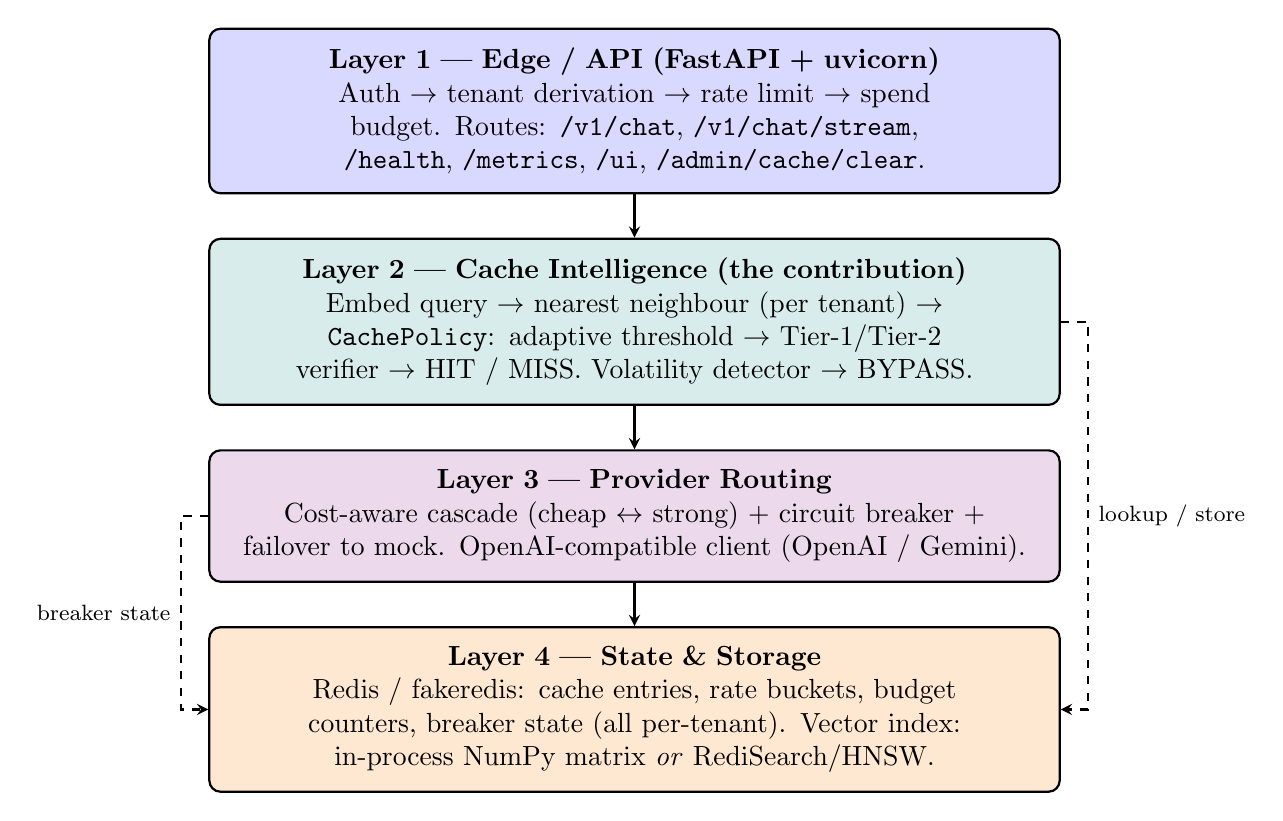
\begin{tikzpicture}[
        node distance=0.55cm,
        layer/.style={
            rectangle, draw=black, thick, text=black,
            text width=0.85\textwidth, align=center, rounded corners,
            minimum height=1.4cm, inner sep=7pt
        },
        arrow/.style={thick, ->, >=stealth, draw=black}
    ]
    \node[layer, fill=blue!15] (edge) {\textbf{Layer 1 --- Edge / API (FastAPI + uvicorn)}\\Auth $\rightarrow$ tenant derivation $\rightarrow$ rate limit $\rightarrow$ spend budget. Routes: \texttt{/v1/chat}, \texttt{/v1/chat/stream}, \texttt{/health}, \texttt{/metrics}, \texttt{/ui}, \texttt{/admin/cache/clear}.};
    \node[layer, fill=teal!15, below=of edge] (cache) {\textbf{Layer 2 --- Cache Intelligence (the contribution)}\\Embed query $\rightarrow$ nearest neighbour (per tenant) $\rightarrow$ \texttt{CachePolicy}: adaptive threshold $\rightarrow$ Tier-1/Tier-2 verifier $\rightarrow$ HIT / MISS. Volatility detector $\rightarrow$ BYPASS.};
    \node[layer, fill=violet!15, below=of cache] (route) {\textbf{Layer 3 --- Provider Routing}\\Cost-aware cascade (cheap $\leftrightarrow$ strong) $+$ circuit breaker $+$ failover to mock. OpenAI-compatible client (OpenAI / Gemini).};
    \node[layer, fill=orange!18, below=of route] (state) {\textbf{Layer 4 --- State \& Storage}\\Redis / fakeredis: cache entries, rate buckets, budget counters, breaker state (all per-tenant). Vector index: in-process NumPy matrix \emph{or} RediSearch/HNSW.};

    \draw[arrow] (edge) -- (cache);
    \draw[arrow] (cache) -- (route);
    \draw[arrow] (route) -- (state);
    \draw[arrow, dashed] (cache.east) -- ++(0.35,0) |- node[right, pos=0.25, font=\footnotesize]{lookup / store} (state.east);
    \draw[arrow, dashed] (route.west) -- ++(-0.35,0) |- node[left, pos=0.25, font=\footnotesize]{breaker state} (state.west);
    \end{tikzpicture}%
    }
    \caption{VeriGate four-layer architecture. Requests descend from the edge; a verified cache hit in Layer~2 short-circuits the provider call in Layer~3. All state in Layer~4 is namespaced per tenant.}
    \label{fig:sys_arch}
\end{figure}

\section{Request Lifecycle and the Cache Decision}
The defining logic of VeriGate is the decision, taken for every query, among four outcomes: \textbf{BYPASS} (volatile, never cached), \textbf{HIT} (a verified equivalent answer is served), \textbf{blocked} (a candidate above threshold is rejected by the verifier and demoted to a miss), and \textbf{MISS} (the provider is called and the answer is stored). Figure~\ref{fig:decision} formalises this flow.

\begin{figure}[H]
    \centering
    \resizebox{0.95\textwidth}{!}{
    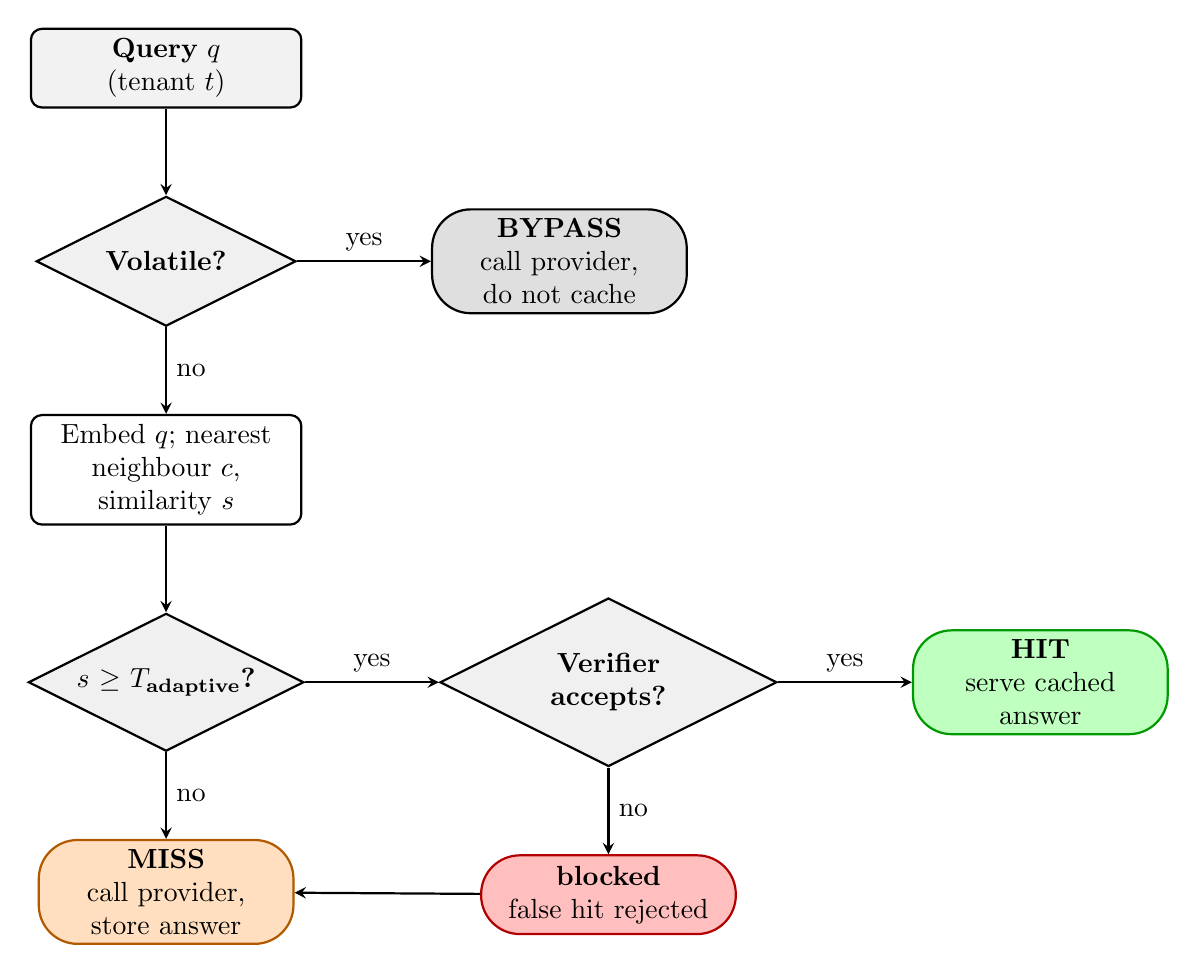
\begin{tikzpicture}[
        node distance=1.1cm and 1.7cm,
        decision/.style={diamond, draw, thick, aspect=2, text width=2.6cm, align=center, inner sep=1pt, fill=gray!12},
        block/.style={rectangle, draw, thick, text width=3.2cm, align=center, rounded corners, minimum height=1cm, fill=white},
        term/.style={rectangle, draw, thick, text width=3.0cm, align=center, rounded corners=14pt, minimum height=1cm},
        arrow/.style={thick, ->, >=stealth}
    ]
    \node[block, fill=gray!10] (in) {\textbf{Query $q$}\\(tenant $t$)};
    \node[decision, below=of in] (vol) {\textbf{Volatile?}};
    \node[term, right=of vol, fill=gray!25] (bypass) {\textbf{BYPASS}\\call provider, do not cache};
    \node[block, below=of vol] (emb) {Embed $q$; nearest neighbour $c$, similarity $s$};
    \node[decision, below=of emb] (thr) {\textbf{$s \geq T_{\text{adaptive}}$?}};
    \node[decision, right=of thr] (ver) {\textbf{Verifier\\accepts?}};
    \node[term, right=of ver, fill=green!25, draw=green!60!black] (hit) {\textbf{HIT}\\serve cached answer};
    \node[term, below=of ver, fill=red!25, draw=red!70!black] (blocked) {\textbf{blocked}\\false hit rejected};
    \node[term, below=of thr, fill=orange!25, draw=orange!70!black] (miss) {\textbf{MISS}\\call provider, store answer};

    \draw[arrow] (in) -- (vol);
    \draw[arrow] (vol) -- node[above]{yes} (bypass);
    \draw[arrow] (vol) -- node[right]{no} (emb);
    \draw[arrow] (emb) -- (thr);
    \draw[arrow] (thr) -- node[above]{yes} (ver);
    \draw[arrow] (thr) -- node[right]{no} (miss);
    \draw[arrow] (ver) -- node[above]{yes} (hit);
    \draw[arrow] (ver) -- node[right]{no} (blocked);
    \draw[arrow] (blocked) -- (miss);
    \end{tikzpicture}
    }
    \caption{The four-outcome cache decision. A candidate whose similarity clears the adaptive threshold is still subjected to the verifier; only a verified candidate is served as a HIT, while a rejected one is demoted to a MISS (``blocked''). Volatile queries bypass the cache entirely.}
    \label{fig:decision}
\end{figure}

\section{Cache Intelligence Design}
The cache intelligence is composed of three sub-designs that together constitute the novel contribution.

\subsection{Adaptive Similarity Threshold}
\label{sec:adaptive}
Rather than a global constant $T_{\text{base}}$, the effective threshold is raised in \emph{dense} neighbourhoods, where many stored queries crowd around the incoming one and the risk of a look-alike collision is highest. Let $s$ be the top-1 cosine similarity and let a local density signal $\rho \in [0,1]$ measure how close the runner-up neighbours are to the top candidate. The adaptive threshold is
\begin{equation}
\label{eq:adaptive}
    T_{\text{adaptive}} = \min\!\big(T_{\max},\; T_{\text{base}} + \alpha \cdot \rho\big),
\end{equation}
where $T_{\text{base}}$ is the calibrated base threshold for the embedding model (0.72 for \texttt{all-MiniLM-L6-v2}, see Chapter~6), $\alpha$ is a sensitivity coefficient, and $T_{\max}$ caps the strictness. In sparse regions the threshold stays near $T_{\text{base}}$ so genuine paraphrases still hit; in dense regions it rises so ambiguous look-alikes are held to a higher bar. This directly attacks the related-topic false hits that a fixed threshold cannot separate without also rejecting paraphrases.

\subsection{Two-Tier Self-Verifier}
\label{sec:verifier}
The verifier is the mechanism that distinguishes VeriGate from all fixed-threshold caches. It runs \emph{after} a candidate clears the threshold and decides whether the two queries truly mean the same thing.

\paragraph{Tier-1 (structural, near-free).} Most dangerous false hits differ in a small set of high-signal features. Tier-1 extracts and compares:
\begin{itemize}
    \item \textbf{Numbers} --- a query mentioning ``5 gb'' must not be served the ``50 gb'' answer;
    \item \textbf{Negation} --- ``how to enable X'' must not be served ``how to disable X'';
    \item \textbf{Named entities} --- ``capital of Austria'' must not be served ``capital of Australia''.
\end{itemize}
If the candidate and the query disagree on any of these, the hit is rejected with a reason code (e.g. \texttt{number\_mismatch}). Tier-1 deliberately does \emph{not} use blanket word-overlap, which an early design showed wrongly rejects legitimate paraphrases that share few words; it checks only the load-bearing tokens.

\paragraph{Tier-2 (NLI, optional).} For correctness-critical domains, an NLI cross-encoder \cite{he2021deberta, bowman2015snli} tests \emph{bidirectional} entailment: the candidate is accepted only if $q \Rightarrow c$ and $c \Rightarrow q$. It is gated behind a configuration flag because it is comparatively expensive and, as Chapter~6 shows, largely redundant once the adaptive threshold is active.

\subsection{Volatility Detection}
\label{sec:volatility}
A volatility classifier flags queries whose correct answer changes with time (weather, prices, ``today'', ``current'', ``now''). Such queries are marked BYPASS: they are never served from and never written to the cache, eliminating the staleness class of errors entirely.

\section{Cost-Aware Cascade Design}
\label{sec:cascade}
For queries that miss the cache, a complexity score $\kappa(q) \in [0,1]$ (based on length, structure, and difficulty cues) decides the model tier: if $\kappa(q) < \tau$ the query is routed to the cheap model, otherwise it is escalated to the strong model. The unused tier is retained as failover. This realises the FrugalGPT cascade idea \cite{chen2023frugalgpt} in a transparent, dependency-free form.

\begin{figure}[H]
    \centering
    \resizebox{0.9\textwidth}{!}{
    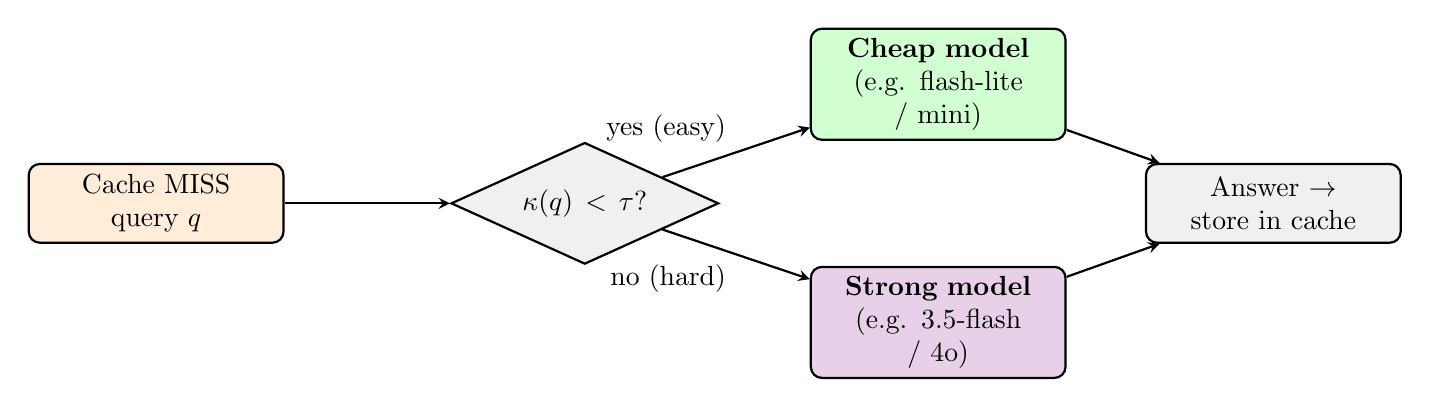
\begin{tikzpicture}[
        node distance=1.2cm and 2.1cm,
        block/.style={rectangle, draw, thick, text width=3.0cm, align=center, rounded corners, minimum height=1cm, fill=white},
        decision/.style={diamond, draw, thick, aspect=2.2, text width=2.4cm, align=center, inner sep=1pt, fill=gray!12},
        arrow/.style={thick, ->, >=stealth}
    ]
    \node[block, fill=orange!15] (miss) {Cache MISS query $q$};
    \node[decision, right=of miss] (score) {$\kappa(q) < \tau$?};
    \node[block, above right=0.4cm and 2cm of score, fill=green!18] (cheap) {\textbf{Cheap model}\\(e.g. flash-lite / mini)};
    \node[block, below right=0.4cm and 2cm of score, fill=violet!18] (strong) {\textbf{Strong model}\\(e.g. 3.5-flash / 4o)};
    \node[block, right=5.4cm of score, fill=gray!12] (ans) {Answer $\rightarrow$ store in cache};
    \draw[arrow] (miss) -- (score);
    \draw[arrow] (score) -- node[above left]{yes (easy)} (cheap);
    \draw[arrow] (score) -- node[below left]{no (hard)} (strong);
    \draw[arrow] (cheap) -- (ans);
    \draw[arrow] (strong) -- (ans);
    \end{tikzpicture}
    }
    \caption{Cost-aware cascade. A transparent complexity score routes easy queries to the cheap model and escalates only hard ones to the strong model; the unused tier remains as a failover.}
    \label{fig:cascade_design}
\end{figure}

\section{Data Model and Tenant Namespacing}
All state is partitioned per tenant to close the cross-tenant leakage risk. The tenant identifier is derived deterministically from the API key so that keys never appear in storage:
\begin{equation}
    \texttt{tenant\_id} = \texttt{"t\_"} + \mathrm{SHA256}(\texttt{api\_key})[{:}16].
\end{equation}
Table~\ref{tab:datamodel} lists the namespaced keys. The in-process index is a dictionary of per-tenant NumPy matrices; the RediSearch backend stores a \texttt{tenant} TAG field and pre-filters every $k$-nearest-neighbour query by it.

\begin{table}[H]
    \centering
    \resizebox{\textwidth}{!}{
    \begin{tabular}{|l|l|l|}
    \hline
    \textbf{Purpose} & \textbf{Key pattern} & \textbf{Notes} \\ \hline
    Cache entry ids & \texttt{cache:ids:<tenant>} & set of entry ids for the tenant \\ \hline
    Cache entry & \texttt{cache:entry:<tenant>:<id>} & stored query, answer, vector; optional TTL \\ \hline
    Rate-limit bucket & \texttt{ratelimit:<api\_key>} & token-bucket state (atomic) \\ \hline
    Spend budget & \texttt{budget:<api\_key>:<day>} & provider-call counter; hits are free \\ \hline
    Circuit breaker & \texttt{breaker:open:<provider>} & open/closed state + failure count \\ \hline
    RediSearch doc & \texttt{vec:<tenant>:<id>} & HNSW-indexed vector with \texttt{tenant} TAG \\ \hline
    \end{tabular}
    }
    \caption{Namespaced state in Redis. Every cache and index key is scoped by \texttt{tenant\_id}, so one tenant can never read another's entries.}
    \label{tab:datamodel}
\end{table}

\section{API Route Design}
\begin{table}[H]
    \centering
    \resizebox{\textwidth}{!}{
    \begin{tabular}{|l|l|l|p{6.2cm}|}
    \hline
    \textbf{Route} & \textbf{Method} & \textbf{Auth} & \textbf{Purpose} \\ \hline
    \texttt{/v1/chat} & POST & Yes & Chat completion (non-streaming JSON) with cache lookup. \\ \hline
    \texttt{/v1/chat/stream} & POST & Yes & Streaming completion (Server-Sent Events). \\ \hline
    \texttt{/health} & GET & No & Liveness + live configuration (backends, provider). \\ \hline
    \texttt{/metrics} & GET & No$^{\dagger}$ & Prometheus metrics (requests, cache outcomes, latency). \\ \hline
    \texttt{/admin/cache/clear} & POST & Yes & Clears \emph{only} the caller's tenant cache. \\ \hline
    \texttt{/} , \texttt{/ui} & GET & No & Operator dashboard (interactive testing). \\ \hline
    \end{tabular}
    }
    \caption{Primary API routes. $^{\dagger}$\,\texttt{/metrics} is public in the demo build and is flagged for lock-down before any multi-tenant public deployment (Chapter~5, security).}
    \label{tab:api_routes}
\end{table}

\section{Failure-Mode and Error-Handling Design}
The gateway is designed to degrade gracefully rather than fail:
\begin{enumerate}
    \item \textbf{Cache fails open.} If Redis or the vector index errors, the request degrades to a normal provider call rather than returning an error --- the cache is an optimisation, never a dependency.
    \item \textbf{Provider failover.} If the selected provider fails (outage, bad key), the router tries the next candidate and finally a mock provider, so a request never hard-fails on a provider problem.
    \item \textbf{Circuit breaker.} After $N$ failures within a window a provider's breaker opens and the router skips it for a cooldown, preventing repeated slow failures against a dead upstream \cite{nygard2018release}.
    \item \textbf{Budget and rate limits.} Over-budget or over-rate requests are rejected cleanly with HTTP~429; cache hits are exempt from the budget so the cache extends, rather than consumes, the allowance.
    \item \textbf{TTL and cleanup.} Optional per-entry TTL bounds memory and self-heals staleness; dangling ids are removed on index rebuild.
\end{enumerate}

        \chapter{Implementation}
        \section{Introduction}
VeriGate is implemented in Python as an asynchronous FastAPI application. This chapter describes the concrete modules, the key engineering decisions and their justifications, and the algorithms that realise the design of Chapter~4. The implementation is organised into the following modules: \texttt{app/main.py} (routes, auth, tenant derivation, rate limit, budget), \texttt{app/config.py} (typed settings), \texttt{app/cache/} (the contribution: \texttt{semantic\_cache.py}, \texttt{policy.py}, \texttt{threshold.py}, \texttt{verifier.py}, \texttt{volatility.py}, \texttt{redisearch\_store.py}), \texttt{app/complexity.py} (cascade routing score), \texttt{app/providers/} (provider abstraction, cascade registry, circuit breaker), \texttt{app/budget.py} (spend budget), \texttt{app/metrics.py} (Prometheus counters), and \texttt{app/static/dashboard.html} (operator UI).

\section{Architectural Decisions}

\paragraph{Why FastAPI + uvicorn rather than Flask?}
The gateway is I/O-bound: most of its time is spent awaiting upstream LLM calls. FastAPI's ASGI foundation \cite{fastapi} allows a single worker to handle many concurrent in-flight requests without threads, and it natively supports streaming responses (Server-Sent Events), which are essential for forwarding token streams from the provider. Pydantic-based request validation rejects malformed bodies with HTTP~422 for free.

\paragraph{Why sentence-transformer embeddings rather than TF-IDF?}
A semantic cache must match by \emph{meaning}. Sparse TF-IDF vectors \cite{salton1988term} encode lexical overlap, so two paraphrases with few shared words are nearly orthogonal and would never hit. Dense sentence embeddings \cite{reimers2019sentencebert} place paraphrases close together regardless of surface form. \texttt{all-MiniLM-L6-v2} \cite{sentencetransformers, wang2020minilm} was chosen for its balance of quality and low CPU latency; a deterministic hash-based lexical embedder is retained purely as a dependency-free fallback for the test suite.

\paragraph{Why an in-process vector index as the default, with RediSearch optional?}
For a single node the fastest possible lookup is a single matrix--vector product held entirely in RAM, with no network hop; this is the default \texttt{inproc} backend. For horizontally-scaled deployments that must share one cache across replicas, or for caches too large for one process's memory, a RediSearch/HNSW backend \cite{malkov2018hnsw, redis_stack} is provided behind a configuration switch. This gives the right default for the common case without foreclosing scale.

\paragraph{Why Redis (with fakeredis) for state?}
Redis provides atomic operations for the rate-limit token bucket and spend counters, TTLs for cache entries, and a shared store for breaker state across replicas. For development and tests, \texttt{fakeredis} offers the same interface in-process with no server to run, so the whole system is exercisable with a single \texttt{pytest} invocation.

\paragraph{Why keep a mock provider permanently in the chain?}
Placing a free mock provider as the terminal failover means a provider outage or a bad key degrades to a valid (if synthetic) response rather than a 500 error, satisfying the graceful-degradation requirement and making the system demonstrable with no API key at all.

\section{Configuration}
All behaviour is controlled by a single typed \texttt{Settings} object (\texttt{pydantic-settings}) read from environment variables, so the same image runs in every environment by changing configuration only. Key knobs include \texttt{REDIS\_URL}, \texttt{CACHE\_SIMILARITY\_BASE} (0.72), \texttt{EMBEDDING\_BACKEND} (\texttt{minilm}/\texttt{hash}), \texttt{VECTOR\_BACKEND} (\texttt{inproc}/\texttt{redisearch}), \texttt{VERIFIER\_NLI} (default off), \texttt{LLM\_PROVIDER}, \texttt{CASCADE\_ENABLED}, \texttt{DAILY\_REQUEST\_BUDGET}, the \texttt{BREAKER\_*} parameters, \texttt{CACHE\_TTL\_SEC}, and \texttt{API\_KEYS}. Critically, the live gateway and the evaluation harness both import the same \texttt{CachePolicy}, so measured behaviour equals shipped behaviour.

\section{The Cache Policy}
The policy is the single decision point of Figure~\ref{fig:decision}. Algorithm~\ref{alg:policy} gives its logic. It is intentionally small and pure so that it can be unit-tested and reused verbatim by the evaluator.

\begin{algorithm}[H]
\caption{Cache decision (\texttt{CachePolicy.decide})}\label{alg:policy}
\begin{algorithmic}[1]
\Require query $q$, candidate $c$, similarity $s$, neighbourhood density $\rho$, tenant $t$
\Ensure outcome $\in \{$HIT, MISS, BYPASS$\}$ with a reason
\If{\Call{IsVolatile}{$q$}}
    \State \Return (BYPASS, \texttt{volatile})
\EndIf
\State $T \gets \min(T_{\max},\ T_{\text{base}} + \alpha\rho)$ \Comment{adaptive threshold, Eq.~\ref{eq:adaptive}}
\If{$c = \varnothing$ \textbf{or} $s < T$}
    \State \Return (MISS, \texttt{below\_threshold})
\EndIf
\If{\textbf{not} \Call{Tier1Verify}{$q, c$}}
    \State \Return (MISS, \texttt{verify\_rejected:<reason>}) \Comment{false hit blocked}
\EndIf
\If{\texttt{VERIFIER\_NLI} \textbf{and not} \Call{Tier2NLI}{$q, c$}}
    \State \Return (MISS, \texttt{nli\_rejected})
\EndIf
\State \Return (HIT, \texttt{verified})
\end{algorithmic}
\end{algorithm}

\subsection{Adaptive Threshold and Calibration}
The base threshold was calibrated empirically. The MiniLM cosine-similarity distribution sits lower than the hash embedder's, so an initial value of 0.82 rejected valid paraphrases; it was recalibrated to \textbf{0.72} (Chapter~6). This is itself evidence for the adaptive design: because the correct threshold is embedding-dependent, hard-coding one is fragile. The adaptive term of Equation~\ref{eq:adaptive} then lifts the threshold in dense neighbourhoods at run time.

\subsection{Tier-1 Structural Verifier}
Algorithm~\ref{alg:verify} compares only the load-bearing tokens. An earlier version used a blanket Jaccard word-overlap check, which wrongly rejected paraphrases sharing few words --- defeating the purpose of semantic matching. The redesign compares numbers, negation state, and named entities only, deferring subtler distinctions to the optional Tier-2 NLI stage.

\begin{algorithm}[H]
\caption{Tier-1 structural verification}\label{alg:verify}
\begin{algorithmic}[1]
\Require query $q$, candidate $c$
\Ensure accept (true) or reject with reason
\If{$\textsc{Numbers}(q) \neq \textsc{Numbers}(c)$}
    \State \Return reject(\texttt{number\_mismatch})
\EndIf
\If{$\textsc{Negated}(q) \neq \textsc{Negated}(c)$}
    \State \Return reject(\texttt{negation\_mismatch})
\EndIf
\If{$\textsc{Entities}(q) \neq \textsc{Entities}(c)$}
    \State \Return reject(\texttt{entity\_mismatch})
\EndIf
\State \Return accept
\end{algorithmic}
\end{algorithm}

\subsection{Tier-2 NLI Verifier}
When \texttt{VERIFIER\_NLI} is enabled, a compact cross-encoder (\texttt{cross-encoder/nli-deberta-v3-xsmall}) \cite{he2021deberta} scores entailment in both directions; the candidate is accepted only if $q\!\Rightarrow\!c$ and $c\!\Rightarrow\!q$. Results are memoised per query pair so that a threshold sweep pays the NLI cost at most once per pair. The performance/recall trade-off that makes this stage opt-in is quantified in Chapter~6.

\section{Semantic Cache and Vector Index}
\label{sec:index}
\texttt{semantic\_cache.py} holds the per-tenant index. \texttt{lookup(query, tenant)} embeds the query and computes the nearest neighbour; \texttt{store(query, answer, tenant)} appends the new vector. The \texttt{inproc} backend keeps, per tenant, one NumPy matrix of stacked unit-normalised vectors, so a lookup is a single matrix--vector product followed by an \texttt{argmax} --- reducing what was an $O(n)$ parse-and-cosine loop to a sub-millisecond operation (Chapter~6, Phase~9). The \texttt{redisearch} backend (\texttt{redisearch\_store.py}) creates an HNSW index with a \texttt{tenant} TAG and issues KNN queries of the form \texttt{(@tenant:\{t\})=>[KNN k @vec \$BLOB]}, so the isolation boundary is enforced inside the index itself.

\section{Provider Abstraction, Cascade, and Circuit Breaker}
A single OpenAI-compatible streaming client (\texttt{openai\_compat.py}) serves both OpenAI and Gemini (via Google's OpenAI-compatibility endpoint), selected by \texttt{LLM\_PROVIDER} and a key read from the environment (never logged). The registry (\texttt{registry.py}) builds either a single provider or, when \texttt{CASCADE\_ENABLED} is set, a cheap/strong pair. \texttt{route\_stream} implements Algorithm~\ref{alg:route}: it scores complexity, orders the tiers, skips any provider whose breaker is open, and always retains the mock as a terminal failover.

\begin{algorithm}[H]
\caption{Cascade routing with breaker and failover}\label{alg:route}
\begin{algorithmic}[1]
\Require query $q$, providers (cheap, strong, mock), threshold $\tau$
\State $\kappa \gets \Call{Complexity}{q}$
\State order $\gets (\kappa < \tau)\ ?\ [\text{cheap, strong, mock}] : [\text{strong, cheap, mock}]$
\For{\textbf{each} provider $P$ \textbf{in} order}
    \If{\Call{BreakerOpen}{$P$}} \State \textbf{continue} \EndIf
    \State try $P$; \textbf{on success} record success, \Return stream
    \State \textbf{on failure} record failure (may open breaker), continue
\EndFor
\end{algorithmic}
\end{algorithm}

The circuit breaker (\texttt{breaker.py}) keeps open/closed state and a failure count in Redis (\texttt{breaker:open:<provider>}), shared across replicas, opening after \texttt{BREAKER\_FAIL\_THRESHOLD} failures within \texttt{BREAKER\_WINDOW\_SEC} and closing after \texttt{BREAKER\_COOLDOWN\_SEC} \cite{nygard2018release}.

\section{Production Hardening}
Three features close pre-deployment blockers identified in the threat model:
\begin{itemize}
    \item \textbf{Per-tenant isolation} --- the cache and index are namespaced by \texttt{tenant\_id}; \texttt{/admin/cache/clear} clears only the caller's tenant. This closes the top vulnerability (cross-tenant leakage).
    \item \textbf{Per-key daily spend budget} (\texttt{budget.py}) --- \texttt{check\_and\_count} increments \texttt{budget:<key>:<day>} and returns over-limit as HTTP~429; \emph{cache hits are never counted}, so the cache extends the budget. This closes the economic-DoS (bill-shock) risk.
    \item \textbf{Cache TTL} (\texttt{CACHE\_TTL\_SEC}) --- optional per-entry expiry bounds memory and self-heals staleness; dangling ids are cleaned on index rebuild.
\end{itemize}

\section{Observability and Operator Dashboard}
\texttt{metrics.py} exposes Prometheus counters and histograms: \texttt{verigate\_requests\_total}, \texttt{verigate\_cache\_total} (by outcome), \texttt{verigate\_false\_hit\_rejected\_total}, \texttt{verigate\_rate\_limited\_total}, \texttt{verigate\_budget\_exceeded\_total}, and \texttt{verigate\_latency\_seconds}. A provisioned Prometheus + Grafana stack (\texttt{docker-compose.observability.yml}) scrapes \texttt{/metrics} and renders a pre-built dashboard. The single-page operator dashboard (\texttt{dashboard.html}), served same-origin at \texttt{/ui}, lets a user ask questions and watch the cache badge (HIT/MISS/BYPASS/blocked), the answer, provider, latency, similarity, threshold, and reason, alongside live session statistics --- the primary interactive demonstration of the contribution.

\section{Testing}
The system ships with an automated \texttt{pytest} suite of \textbf{18 tests} covering the gateway, verifier, cascade, and hardening. \texttt{conftest.py} pins a deterministic configuration (\texttt{EMBEDDING\_BACKEND=hash}, \texttt{VERIFIER\_NLI=false}, \texttt{LLM\_PROVIDER=mock}, \texttt{VECTOR\_BACKEND=inproc}) so tests are fast and reproducible.
\begin{itemize}
    \item \textbf{Unit:} the verifier rejects number/entity/negation mismatches and accepts genuine paraphrases; the complexity scorer routes easy versus hard queries correctly.
    \item \textbf{Integration:} auth returns 401 without a key; a paraphrase produces a HIT after a MISS; a look-alike above threshold is blocked; a volatile query bypasses; a burst is rate-limited (429).
    \item \textbf{Security / hardening:} \texttt{test\_tenant\_isolation} confirms tenant~B cannot read tenant~A's cache; the budget blocks over-limit while keeping hits free; the breaker opens after repeated failures and failover still succeeds.
\end{itemize}
All 18 tests pass in the reference environment, and the same components are exercised through the container image (Chapter~6).

        \chapter{Results and Evaluation}
        \section{Introduction}
This chapter reports the evaluation of VeriGate: functional and test verification, the headline correctness result (false-hit elimination) with its ablation, the mechanism by failure mode, the Tier-2 NLI trade-off, the latency and vector-index results, the backend comparison, the cost-aware cascade, the security (tenant-isolation) result, the live LLM demonstration, observability, and the operator dashboard. Every figure and table is regenerable from the repository, and the evaluation harness shares the exact \texttt{CachePolicy} used by the live gateway, so measured behaviour equals shipped behaviour.

\subsection{Test-Suite Verification}
The automated suite is the first line of evidence that each component behaves as specified. All \textbf{18 tests pass} in the reference environment (Python~3.13, Windows~11).

\begin{table}[H]
    \centering
    \caption{Representative automated tests and the guarantee each proves.}
    \label{tab:tests}
    \footnotesize
    \begin{tabular}{|l|p{8.2cm}|l|}
    \hline
    \textbf{Test} & \textbf{Guarantee proven} & \textbf{Result} \\ \hline
    test\_health & server boots and reports live configuration & PASS \\ \hline
    test\_auth\_required & requests without a valid key are rejected (401) & PASS \\ \hline
    test\_cache\_miss\_then\_hit & a paraphrase is served from cache after the first miss & PASS \\ \hline
    test\_verifier\_rejects\_number\_mismatch & a look-alike differing by a number is NOT served & PASS \\ \hline
    test\_volatile\_query\_bypasses\_cache & time-sensitive queries are never cached & PASS \\ \hline
    test\_rate\_limit\_returns\_429 & a burst is throttled & PASS \\ \hline
    test\_tenant\_isolation & tenant B cannot read tenant A's cached answer & PASS \\ \hline
    test\_cascade\_routing & easy$\rightarrow$cheap, hard$\rightarrow$strong routing is correct & PASS \\ \hline
    test\_budget\_blocks\_over\_limit & over-budget calls are 429; cache hits stay free & PASS \\ \hline
    test\_metrics\_endpoint & Prometheus metrics are exposed & PASS \\ \hline
    \end{tabular}
\end{table}

\section{Headline Result: Eliminating False Hits}
The primary success metric is the false-hit rate --- how often the cache serves a wrong answer to a look-alike query. VeriGate was compared against a fixed-threshold baseline (GPTCache-style, $T=0.72$) on the curated benchmark, adding one component at a time. Table~\ref{tab:ablation} gives the ablation.

\begin{table}[H]
\centering
\caption{Ablation on the benchmark. VeriGate serves zero wrong answers (100\% precision) versus the baseline's 46.7\% false-hit rate.}
\label{tab:ablation}
\begin{tabular}{|l|c|c|c|c|}
\hline
\textbf{System} & \textbf{Hit-rate} & \textbf{False-hit rate} & \textbf{Precision} & \textbf{F1} \\ \hline
Baseline (static $T=0.72$)       & 40.0\% & 46.7\% & 46.2\% & 0.43 \\ \hline
\ \ + Adaptive threshold         & 33.3\% & 33.3\% & 50.0\% & 0.40 \\ \hline
\ \ + Verifier (Tier-1)          & 40.0\% & 13.3\% & 75.0\% & 0.52 \\ \hline
\textbf{VeriGate (full)}         & 33.3\% & \textbf{0.0\%} & \textbf{100.0\%} & 0.50 \\ \hline
\end{tabular}
\end{table}

The baseline serves a wrong answer on nearly half of the hard negatives. VeriGate serves \textbf{none}: it is stricter, so its raw hit-rate is slightly lower, which is the intended and correct trade-off for a system whose priority is correctness. Figure~\ref{fig:tradeoff} makes the trade-off visual.

\begin{figure}[H]
    \centering
    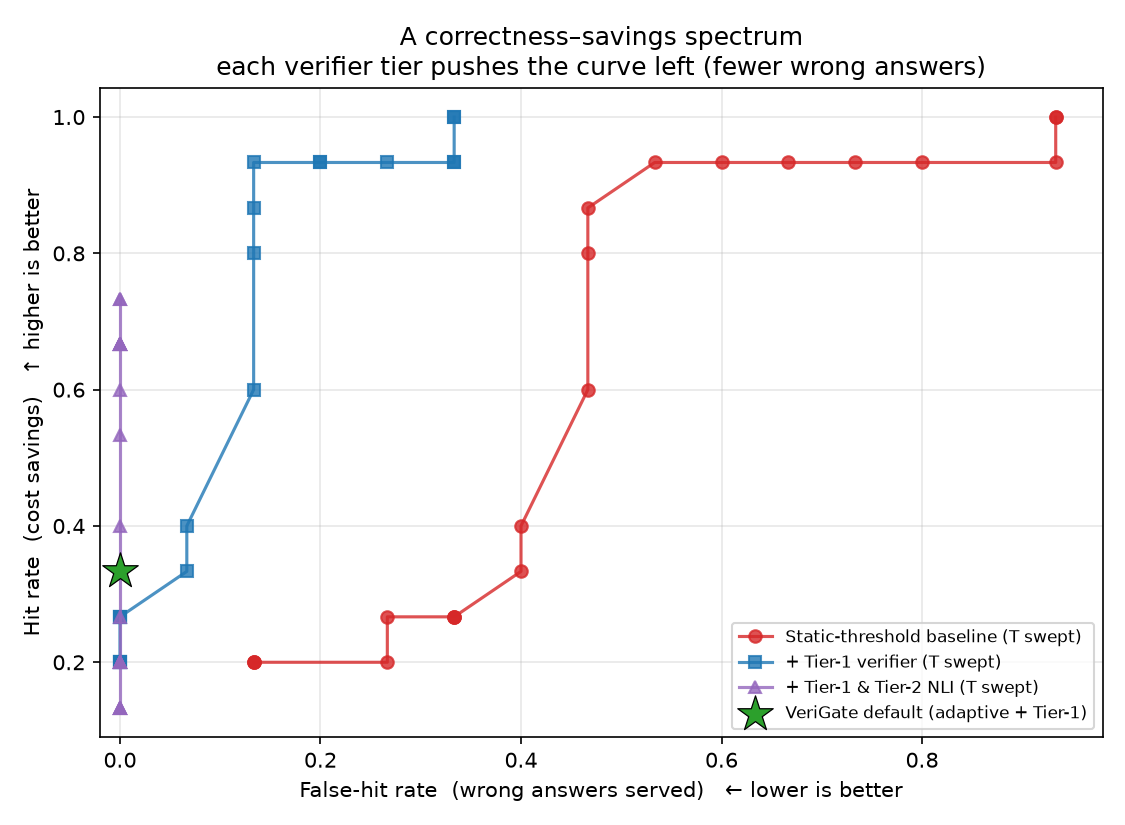
\includegraphics[width=0.82\textwidth,height=0.32\textheight,keepaspectratio]{tradeoff.png}
    \caption{The trade-off (``money'') curve. Sweeping the similarity threshold, false-hit rate (x, lower is better) is plotted against hit-rate (y, higher is better) for the baseline (red) and the verifier-enabled system (blue); the green star is full VeriGate. The blue curve lies \emph{above and to the left} of the red one --- at any hit-rate it serves far fewer wrong answers (Pareto domination).}
    \label{fig:tradeoff}
\end{figure}

\begin{figure}[H]
    \centering
    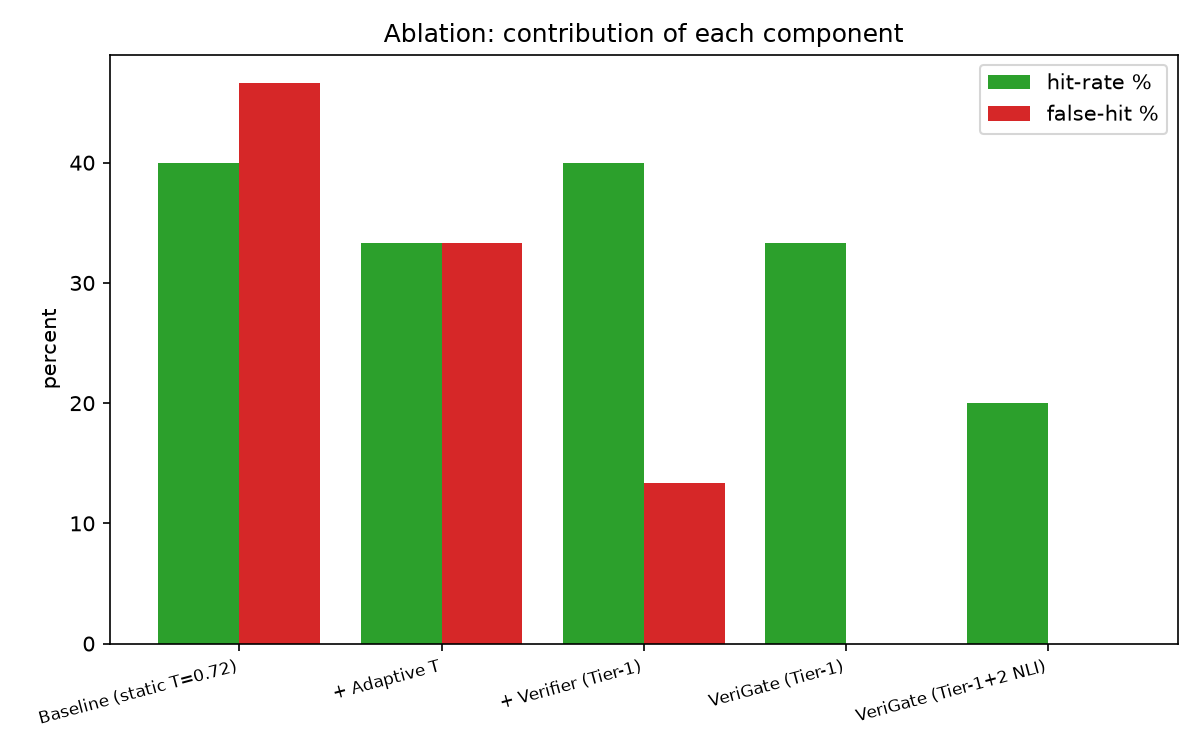
\includegraphics[width=0.82\textwidth,height=0.30\textheight,keepaspectratio]{ablation.png}
    \caption{Ablation bars: hit-rate (green) and false-hit rate (red) as components are added. False-hit rate falls step-by-step to zero for full VeriGate while hit-rate stays reasonable.}
    \label{fig:ablation}
\end{figure}

\subsection{False Hits by Failure Mode (the Mechanism)}
Table~\ref{tab:modes} decomposes the false hits by trap type, showing precisely which component neutralises each. The \emph{verifier} eliminates entity-, number-, and negation-swap false hits; the \emph{adaptive threshold} clears the related-topic ones; together they reach zero.

\begin{table}[H]
    \centering
    \caption{False hits by failure mode (lower is better). Cells show false hits / traps of that type.}
    \label{tab:modes}
    \begin{tabular}{|l|c|c|c|c|}
    \hline
    \textbf{System} & \textbf{entity\_swap} & \textbf{number\_swap} & \textbf{negation} & \textbf{related\_topic} \\ \hline
    Baseline           & 0/5 & 3/3 & 2/2 & 2/5 \\ \hline
    \ \ + Adaptive     & 0/5 & 3/3 & 2/2 & 0/5 \\ \hline
    \ \ + Verifier     & 0/5 & 0/3 & 0/2 & 2/5 \\ \hline
    \textbf{VeriGate}  & 0/5 & \textbf{0/3} & \textbf{0/2} & \textbf{0/5} \\ \hline
    \end{tabular}
\end{table}

\subsection{Volatility (Staleness) Detector}
On the volatility set the detector achieved \textbf{5/5 recall} on volatile queries (all correctly bypassed) with \textbf{0/4 false positives} on stable controls, removing the staleness class of errors entirely.

\section{Tier-2 NLI: A Correctness--Recall Trade-off}
Adding the optional Tier-2 NLI verifier was evaluated in isolation (Table~\ref{tab:nli}).

\begin{table}[H]
    \centering
    \caption{Effect of adding Tier-2 NLI to the full system.}
    \label{tab:nli}
    \begin{tabular}{|l|c|c|c|c|}
    \hline
    \textbf{System} & \textbf{Hit-rate} & \textbf{False-hit} & \textbf{Precision} & \textbf{F1} \\ \hline
    VeriGate (Tier-1)           & 33.3\% & 0.0\% & 100.0\% & 0.50 \\ \hline
    VeriGate (Tier-1 + Tier-2)  & 20.0\% & 0.0\% & 100.0\% & 0.33 \\ \hline
    \end{tabular}
\end{table}

Tier-2 achieves zero false hits at \emph{every} threshold but caps recall lower, because NLI is conservative and rejects some genuine paraphrases. Crucially, it is \textbf{largely redundant once the adaptive threshold is active} --- both target the same related-topic negatives. The design conclusion, a defensible engineering decision rather than a naive ``add more components'' story, is: \emph{the recommended default is adaptive + Tier-1 (zero false hits at higher recall), with Tier-2 offered as an opt-in ``max-correctness mode''} for correctness-critical domains (medical, legal, finance) or when the base threshold must be kept loose.

\section{Latency and the Cache-Hit Path}
Per-stage latency was measured to answer the direct question: \emph{how much does the verification that constitutes the contribution actually cost?}

\begin{table}[H]
    \centering
    \caption{Per-stage latency (milliseconds). Tier-1 verification is effectively free; Tier-2 NLI is a deliberate opt-in cost.}
    \label{tab:latency}
    \begin{tabular}{|l|c|c|c|}
    \hline
    \textbf{Stage} & \textbf{p50} & \textbf{p95} & \textbf{p99} \\ \hline
    Embed query                    & 19.0  & 30.3  & 84.4 \\ \hline
    KNN lookup --- 100 entries     & 27.1  & 35.9  & 41.2 \\ \hline
    KNN lookup --- 1000 entries    & 292.9 & 346.8 & 422.8 \\ \hline
    \textbf{Tier-1 verify}         & \textbf{0.03} & 0.03 & 0.05 \\ \hline
    \textbf{Tier-2 NLI verify}     & \textbf{171.7} & 183.5 & 187.9 \\ \hline
    HIT path (embed+KNN@1000+Tier-1) & 334.3 & 374.0 & 399.3 \\ \hline
    \end{tabular}
\end{table}

\textbf{RQ (verification overhead):} Tier-1 costs $\sim$0.03~ms --- structural safety is effectively free on the hit path. Tier-2 NLI adds $\sim$172~ms, a second reason it is opt-in. Table~\ref{tab:latency} also exposes the real bottleneck in the naive design: the brute-force $O(n)$ KNN scan, which grows to $\sim$293~ms at 1000 entries.

\begin{figure}[H]
    \centering
    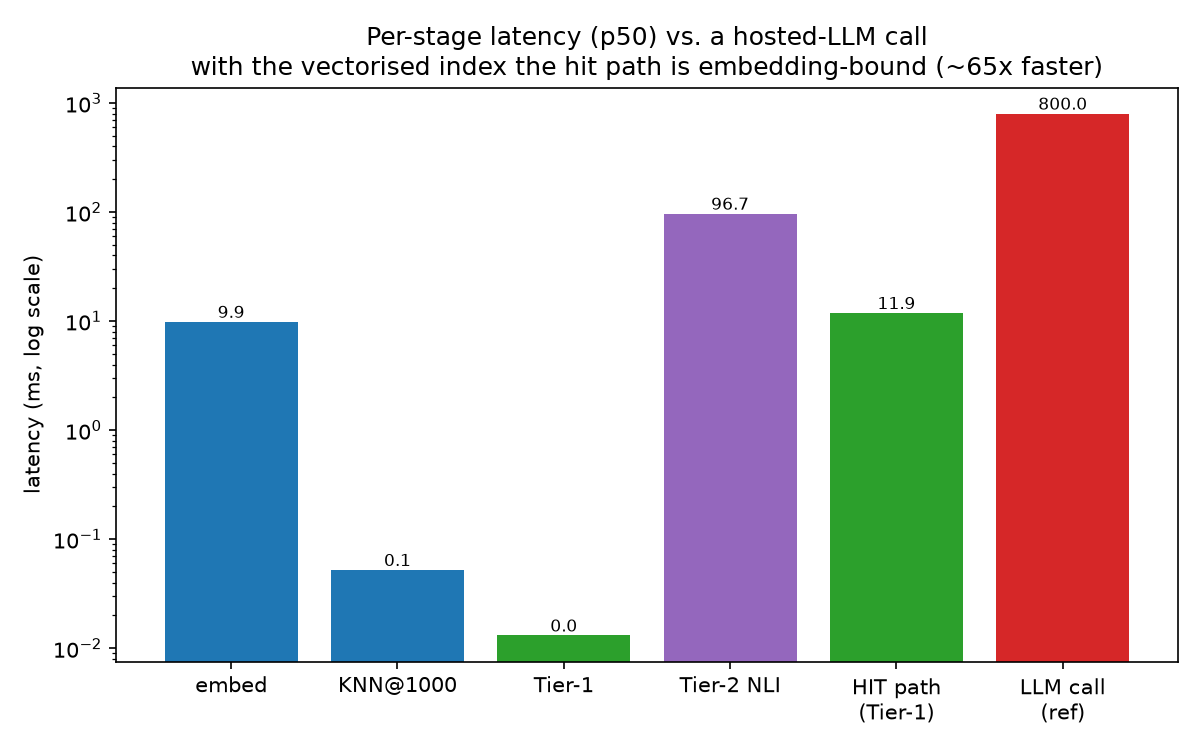
\includegraphics[width=0.82\textwidth,height=0.30\textheight,keepaspectratio]{latency.png}
    \caption{Per-stage latency (log scale) against an 800~ms hosted-LLM reference. Tier-1 verification is invisible ($\sim$free); the costly stages are the NLI check and the KNN scan, both still below the LLM reference.}
    \label{fig:latency}
\end{figure}

\subsection{Vector-Index Upgrade}
The $O(n)$ scan was replaced by a vectorised in-process index (one NumPy matrix, a single matrix--vector product). Table~\ref{tab:index} shows the effect.

\begin{table}[H]
    \centering
    \caption{KNN lookup latency before and after the vectorised index.}
    \label{tab:index}
    \begin{tabular}{|l|c|c|c|}
    \hline
    \textbf{Cache size} & \textbf{Before (parse loop)} & \textbf{After (vectorised)} & \textbf{Speedup} \\ \hline
    1000 entries & $\sim$293 ms & \textbf{0.04 ms} & $\sim$7{,}000$\times$ \\ \hline
    5000 entries & $\sim$1.5 s (extrap.) & \textbf{0.11 ms} & --- \\ \hline
    \end{tabular}
\end{table}

After the upgrade the full cache-hit path is \textbf{$\sim$10~ms} --- about \textbf{78$\times$} faster than an 800~ms LLM call --- and is now bounded by the embedding step, not the lookup. Figure~\ref{fig:scaling} shows lookup staying sub-millisecond and near-flat as the cache grows.

\begin{figure}[H]
    \centering
    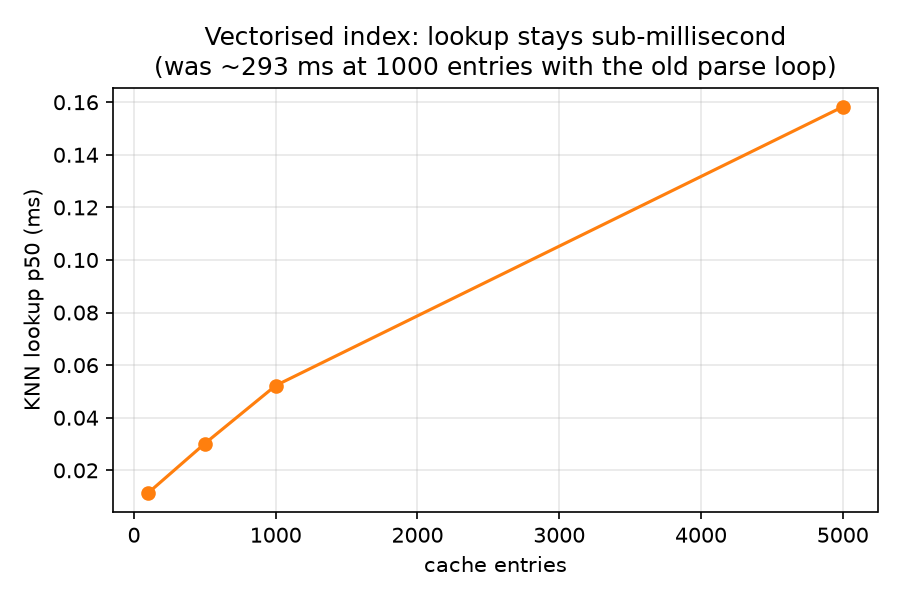
\includegraphics[width=0.82\textwidth,height=0.30\textheight,keepaspectratio]{latency_scaling.png}
    \caption{KNN lookup latency versus cache size. The vectorised in-process index stays sub-millisecond and near-flat to 5000 entries, versus $\sim$293~ms at 1000 for the original parse loop.}
    \label{fig:scaling}
\end{figure}

\subsection{Backend Comparison (In-Process vs RediSearch)}
The RediSearch/HNSW backend was verified end-to-end on a live Redis Stack (a semantic paraphrase HIT and the Austria/Australia trap rejected, both served from the shared index). Table~\ref{tab:backend} compares raw latency.

\begin{table}[H]
    \centering
    \caption{KNN latency (p50): in-process NumPy versus RediSearch/HNSW.}
    \label{tab:backend}
    \begin{tabular}{|l|c|c|}
    \hline
    \textbf{Cache size} & \textbf{In-process (NumPy)} & \textbf{RediSearch (HNSW)} \\ \hline
    1000  & 0.06 ms & 3.60 ms \\ \hline
    5000  & 0.15 ms & 3.83 ms \\ \hline
    10000 & 0.24 ms & 4.69 ms \\ \hline
    \end{tabular}
\end{table}

\begin{figure}[H]
    \centering
    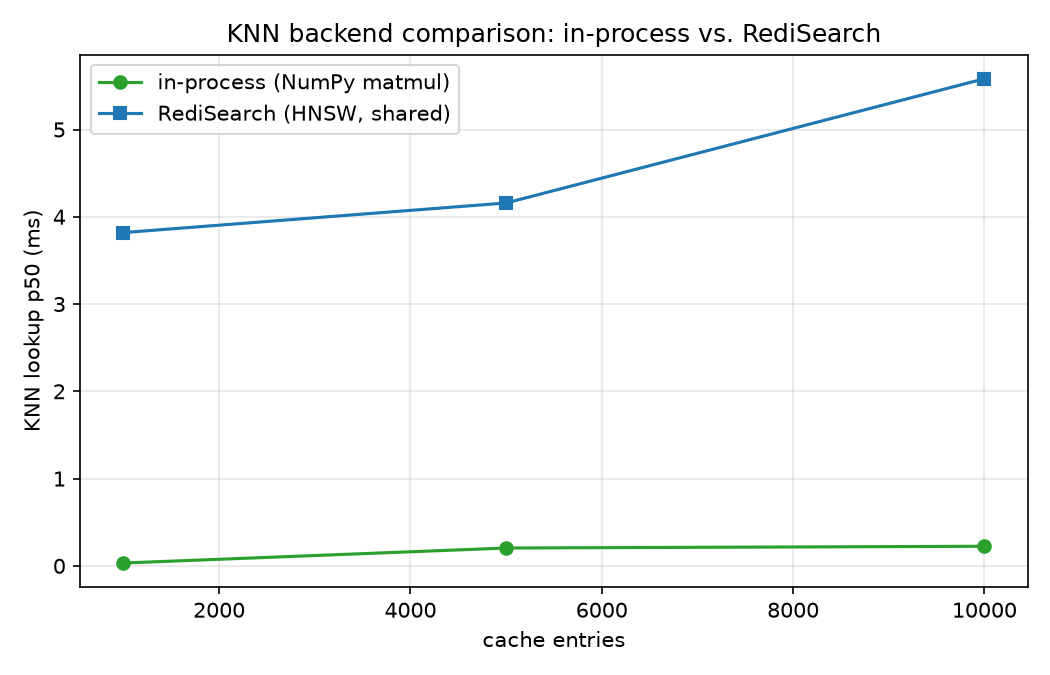
\includegraphics[width=0.80\textwidth,height=0.30\textheight,keepaspectratio]{backend_compare.png}
    \caption{In-process versus RediSearch KNN latency. The in-process index wins on raw latency (no network hop); RediSearch carries a $\sim$3.6~ms round-trip floor but stays nearly flat as the cache grows and is shared across replicas. Both are two-to-four orders of magnitude faster than an LLM call. Recommendation: in-process for a single node, RediSearch for horizontal scale.}
    \label{fig:backend}
\end{figure}

\section{Cost-Aware Cascade}
The second contribution was evaluated by measuring cost reduction against quality retention (cheap cost = 1, strong cost = 15$\times$). Table~\ref{tab:cascade} and Figure~\ref{fig:cascade} give the result.

\begin{table}[H]
    \centering
    \caption{Cascade cost versus quality across routing thresholds.}
    \label{tab:cascade}
    \begin{tabular}{|c|c|c|c|c|c|}
    \hline
    \textbf{Threshold} & \textbf{Escalated} & \textbf{Cost reduction} & \textbf{Quality retained} & \textbf{vs random} & \textbf{Routing F1} \\ \hline
    0.30            & 50\% & \textbf{47\%} & \textbf{100\%} & 50\% & \textbf{1.00} \\ \hline
    0.35 (default)  & $\sim$45\% & $\sim$52\% & $\sim$95\% & $\sim$45\% & $\sim$0.95 \\ \hline
    0.50            & 42\% & 54\% & 85\% & 42\% & 0.92 \\ \hline
    0.70            & 18\% & 77\% & 35\% & 18\% & 0.52 \\ \hline
    \end{tabular}
\end{table}

At threshold~0.30 the cascade cuts LLM cost by \textbf{$\sim$47\%} with \textbf{100\% quality retained} on hard queries, and it sits above random routing at every cost level --- a hard query is far likelier to be escalated than under random routing.

\begin{figure}[H]
    \centering
    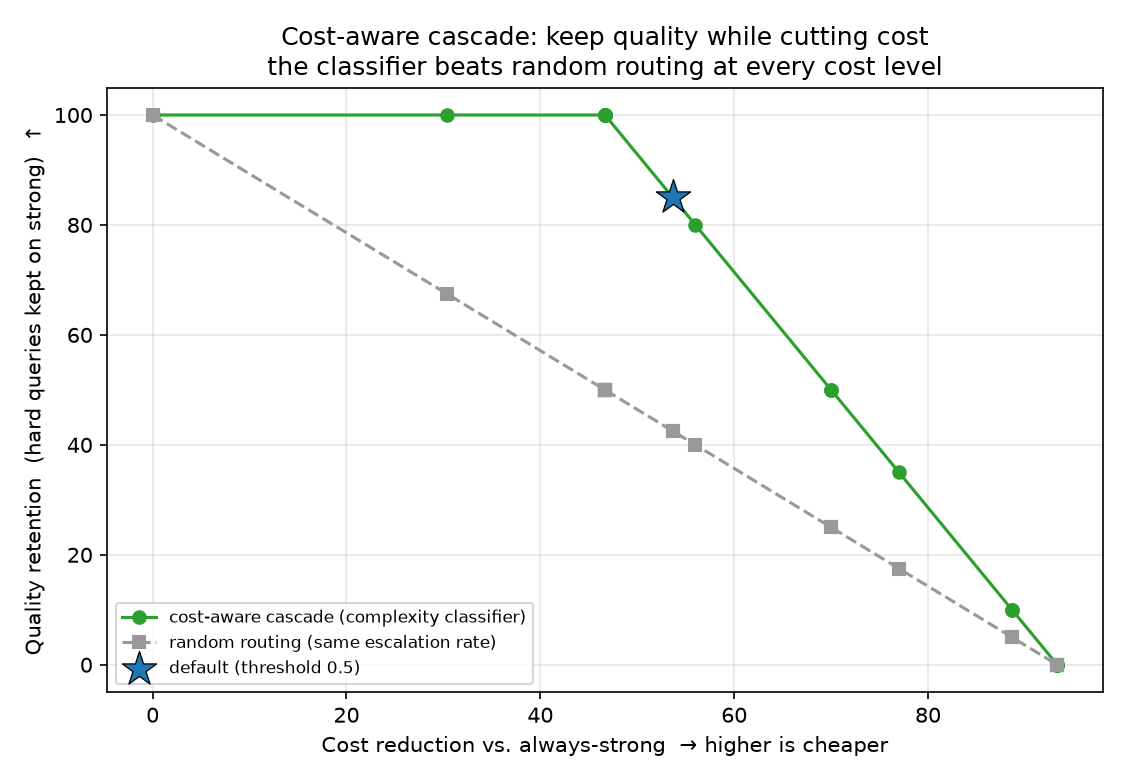
\includegraphics[width=0.80\textwidth,height=0.30\textheight,keepaspectratio]{cascade.png}
    \caption{Quality retention versus cost reduction. The complexity classifier holds 100\% quality up to $\sim$47\% cost reduction, then declines, and dominates random routing at every operating point.}
    \label{fig:cascade}
\end{figure}

\section{Security: Cross-Tenant Isolation}
The threat model identified cross-tenant cache leakage as the single most serious risk of a semantic cache. After partitioning the cache per tenant, tenant~B asking tenant~A's \emph{exact} question receives a \textbf{MISS} (its own empty cache), while A re-asking receives a HIT --- verified in-process by \texttt{test\_tenant\_isolation} and, on the RediSearch backend, by a smoke-test assertion that \texttt{t\_other} cannot retrieve \texttt{t\_demo}'s entry. The defining vulnerability of the design was thus identified and then eliminated with a regression test guarding it.

\section{Live LLM Demonstration}
With a real Gemini key, the gateway returned genuine Gemini answers and then served repeats and paraphrases from cache (Table~\ref{tab:live}). This is the whole thesis on a real model: a slow, paid call becomes an instant, free cache hit --- even for a reworded question.

\begin{table}[H]
    \centering
    \caption{Live gateway with Gemini: first call versus subsequent cache hits.}
    \label{tab:live}
    \begin{tabular}{|l|l|c|p{5.2cm}|}
    \hline
    \textbf{Cache} & \textbf{Provider} & \textbf{Latency} & \textbf{Query} \\ \hline
    MISS & gemini & 23{,}048 ms & ``what is a semantic cache'' (real Gemini call) \\ \hline
    HIT  & cache  & 22 ms & ``what is a semantic cache'' ($\sim$1000$\times$ faster, \$0) \\ \hline
    HIT  & cache  & 20 ms & ``explain what a semantic cache is'' (paraphrase matched by meaning) \\ \hline
    \end{tabular}
\end{table}

\section{Observability}
The provisioned Prometheus + Grafana stack was verified live: the Prometheus target was healthy and Grafana rendered the cache-hit-rate gauge at \textbf{51.1\%} (24 hits / 47 requests) alongside request-rate, cache-outcome, and p95-latency panels driven by real traffic --- demonstrating that the same metrics used for evaluation are exposed for production monitoring.

\section{Operator Dashboard (User Interface) Results}
The gateway serves a single-page operator dashboard at \texttt{/ui} for interactive testing. Figure~\ref{fig:ui_hero} shows the landing view; Figure~\ref{fig:ui_hit} shows a paraphrase served as a HIT; and Figure~\ref{fig:ui_blocked} shows the single clearest proof of the contribution --- a look-alike whose similarity (0.944) is \emph{above} the threshold (0.791) yet is rejected with \texttt{verify\_rejected:number\_mismatch}.

\begin{figure}[H]
    \centering
    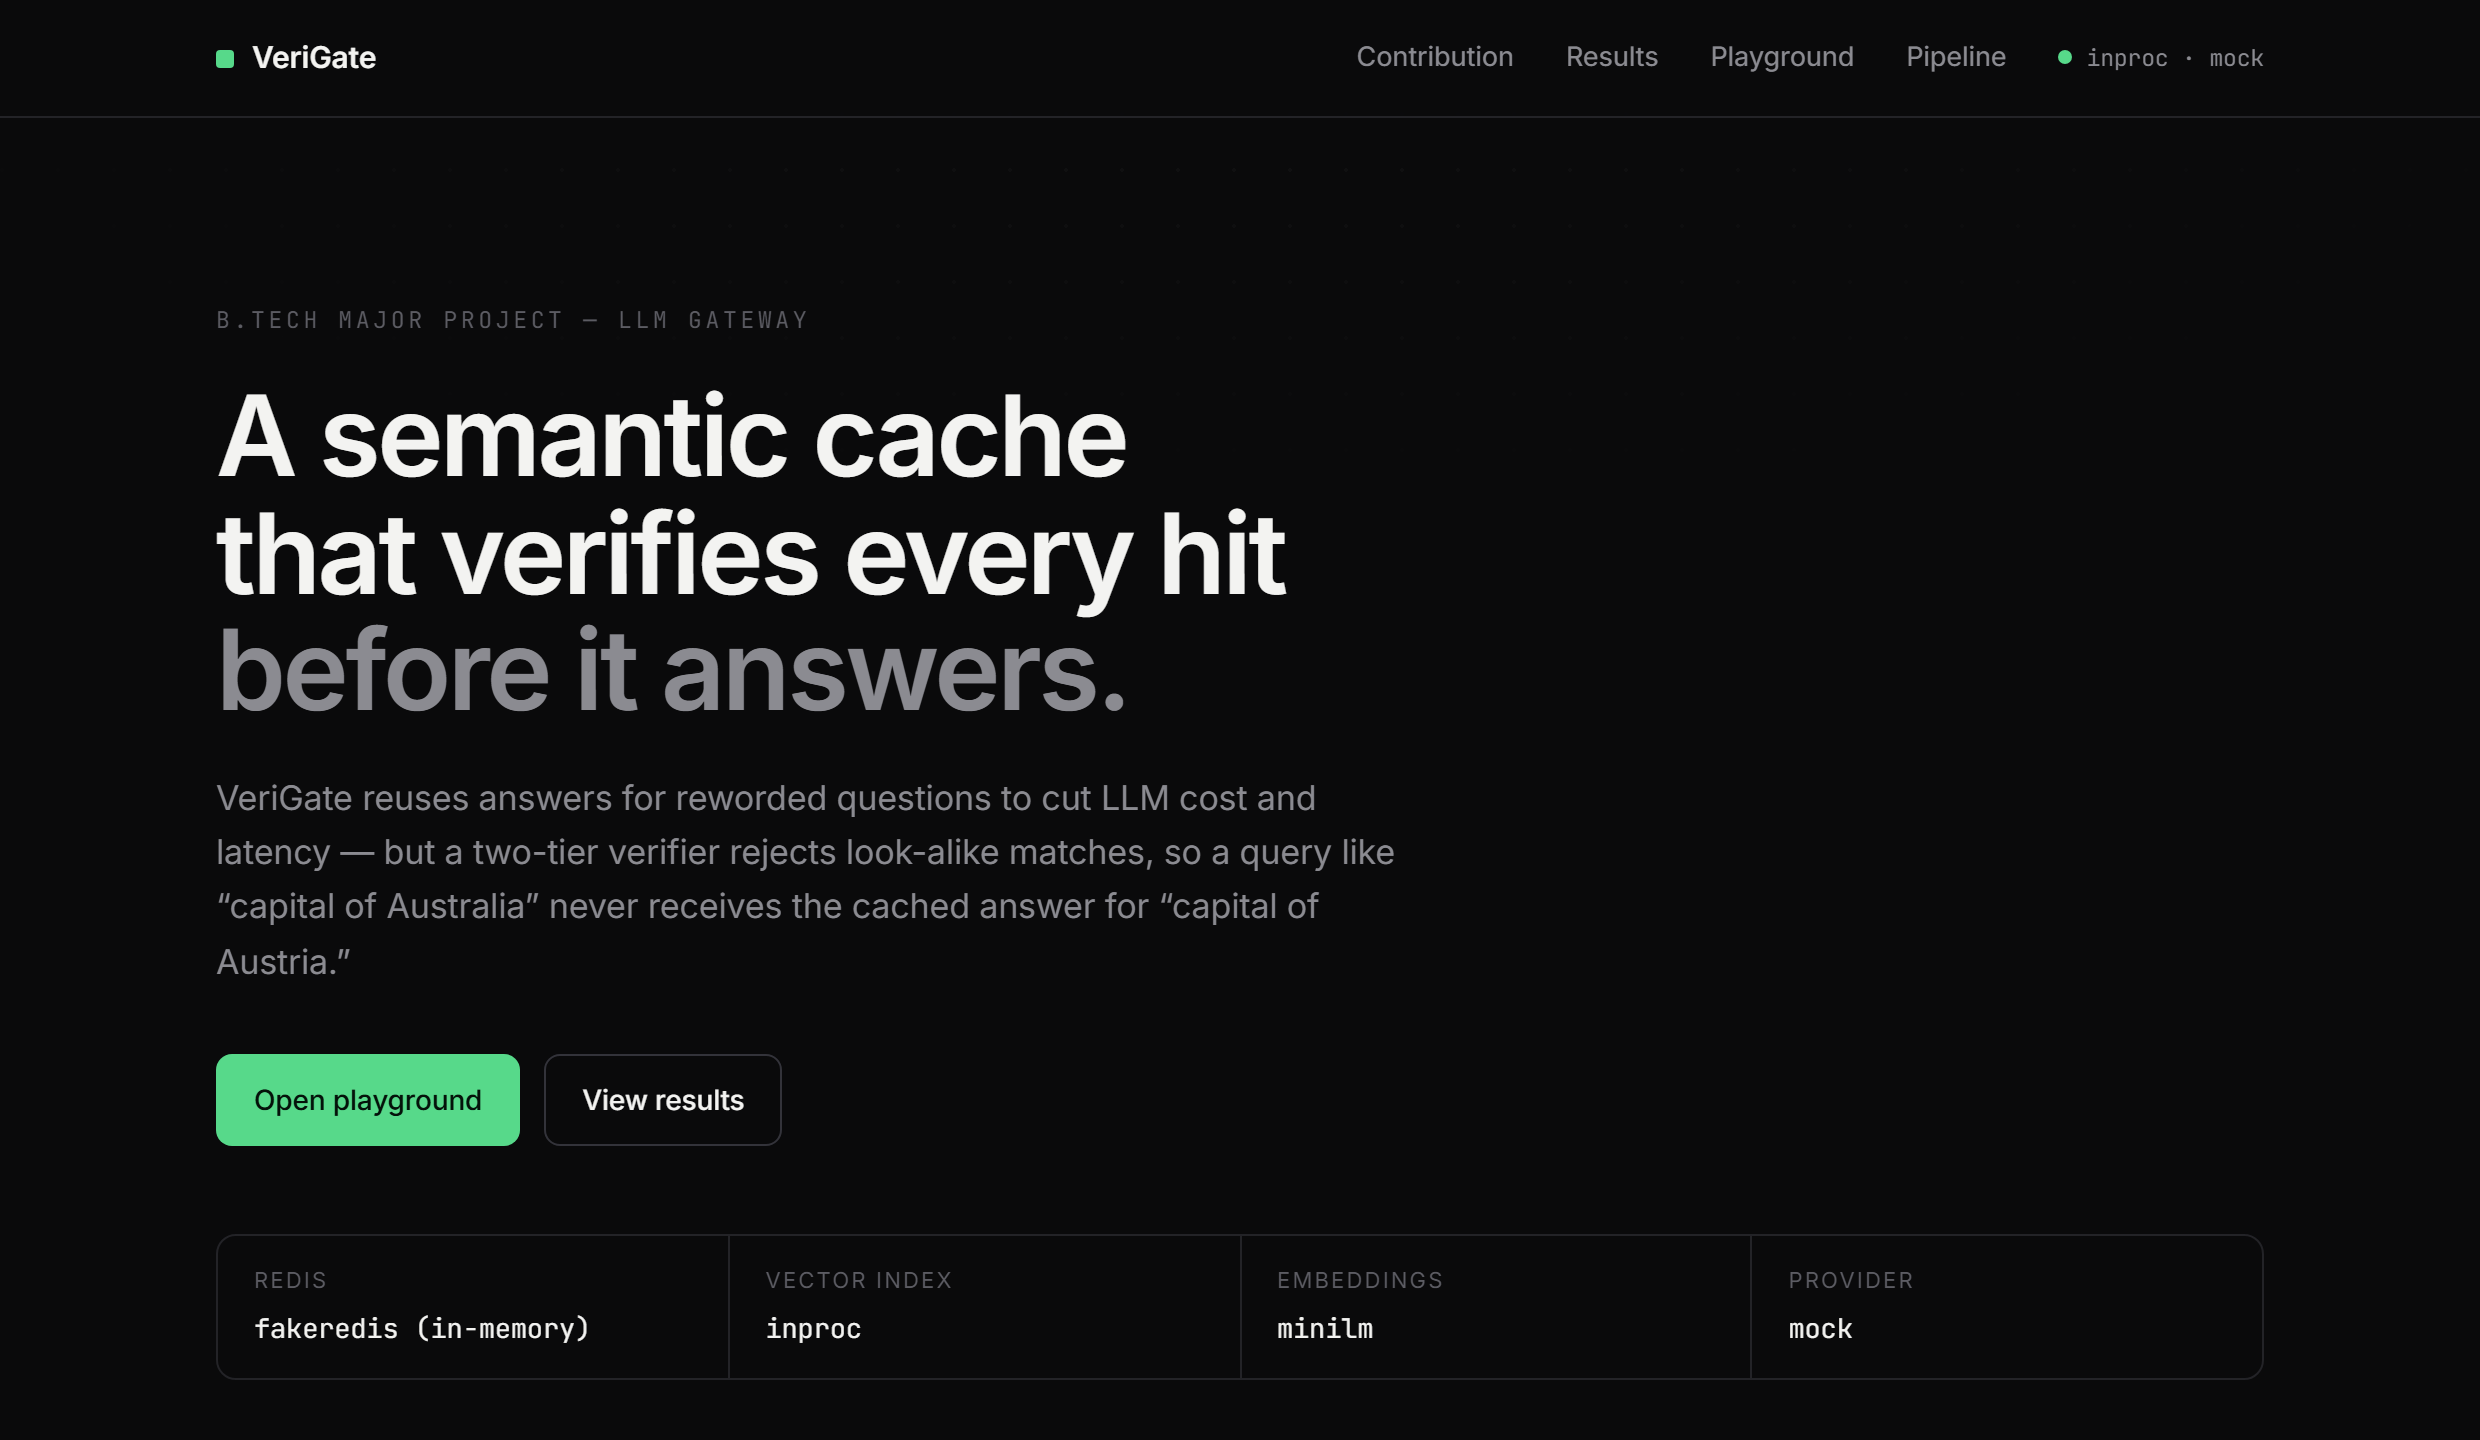
\includegraphics[width=0.90\textwidth]{ui_hero.png}
    \caption{VeriGate operator dashboard --- landing view. The header reports the live configuration (in-process index, mock provider).}
    \label{fig:ui_hero}
\end{figure}

\begin{figure}[H]
    \centering
    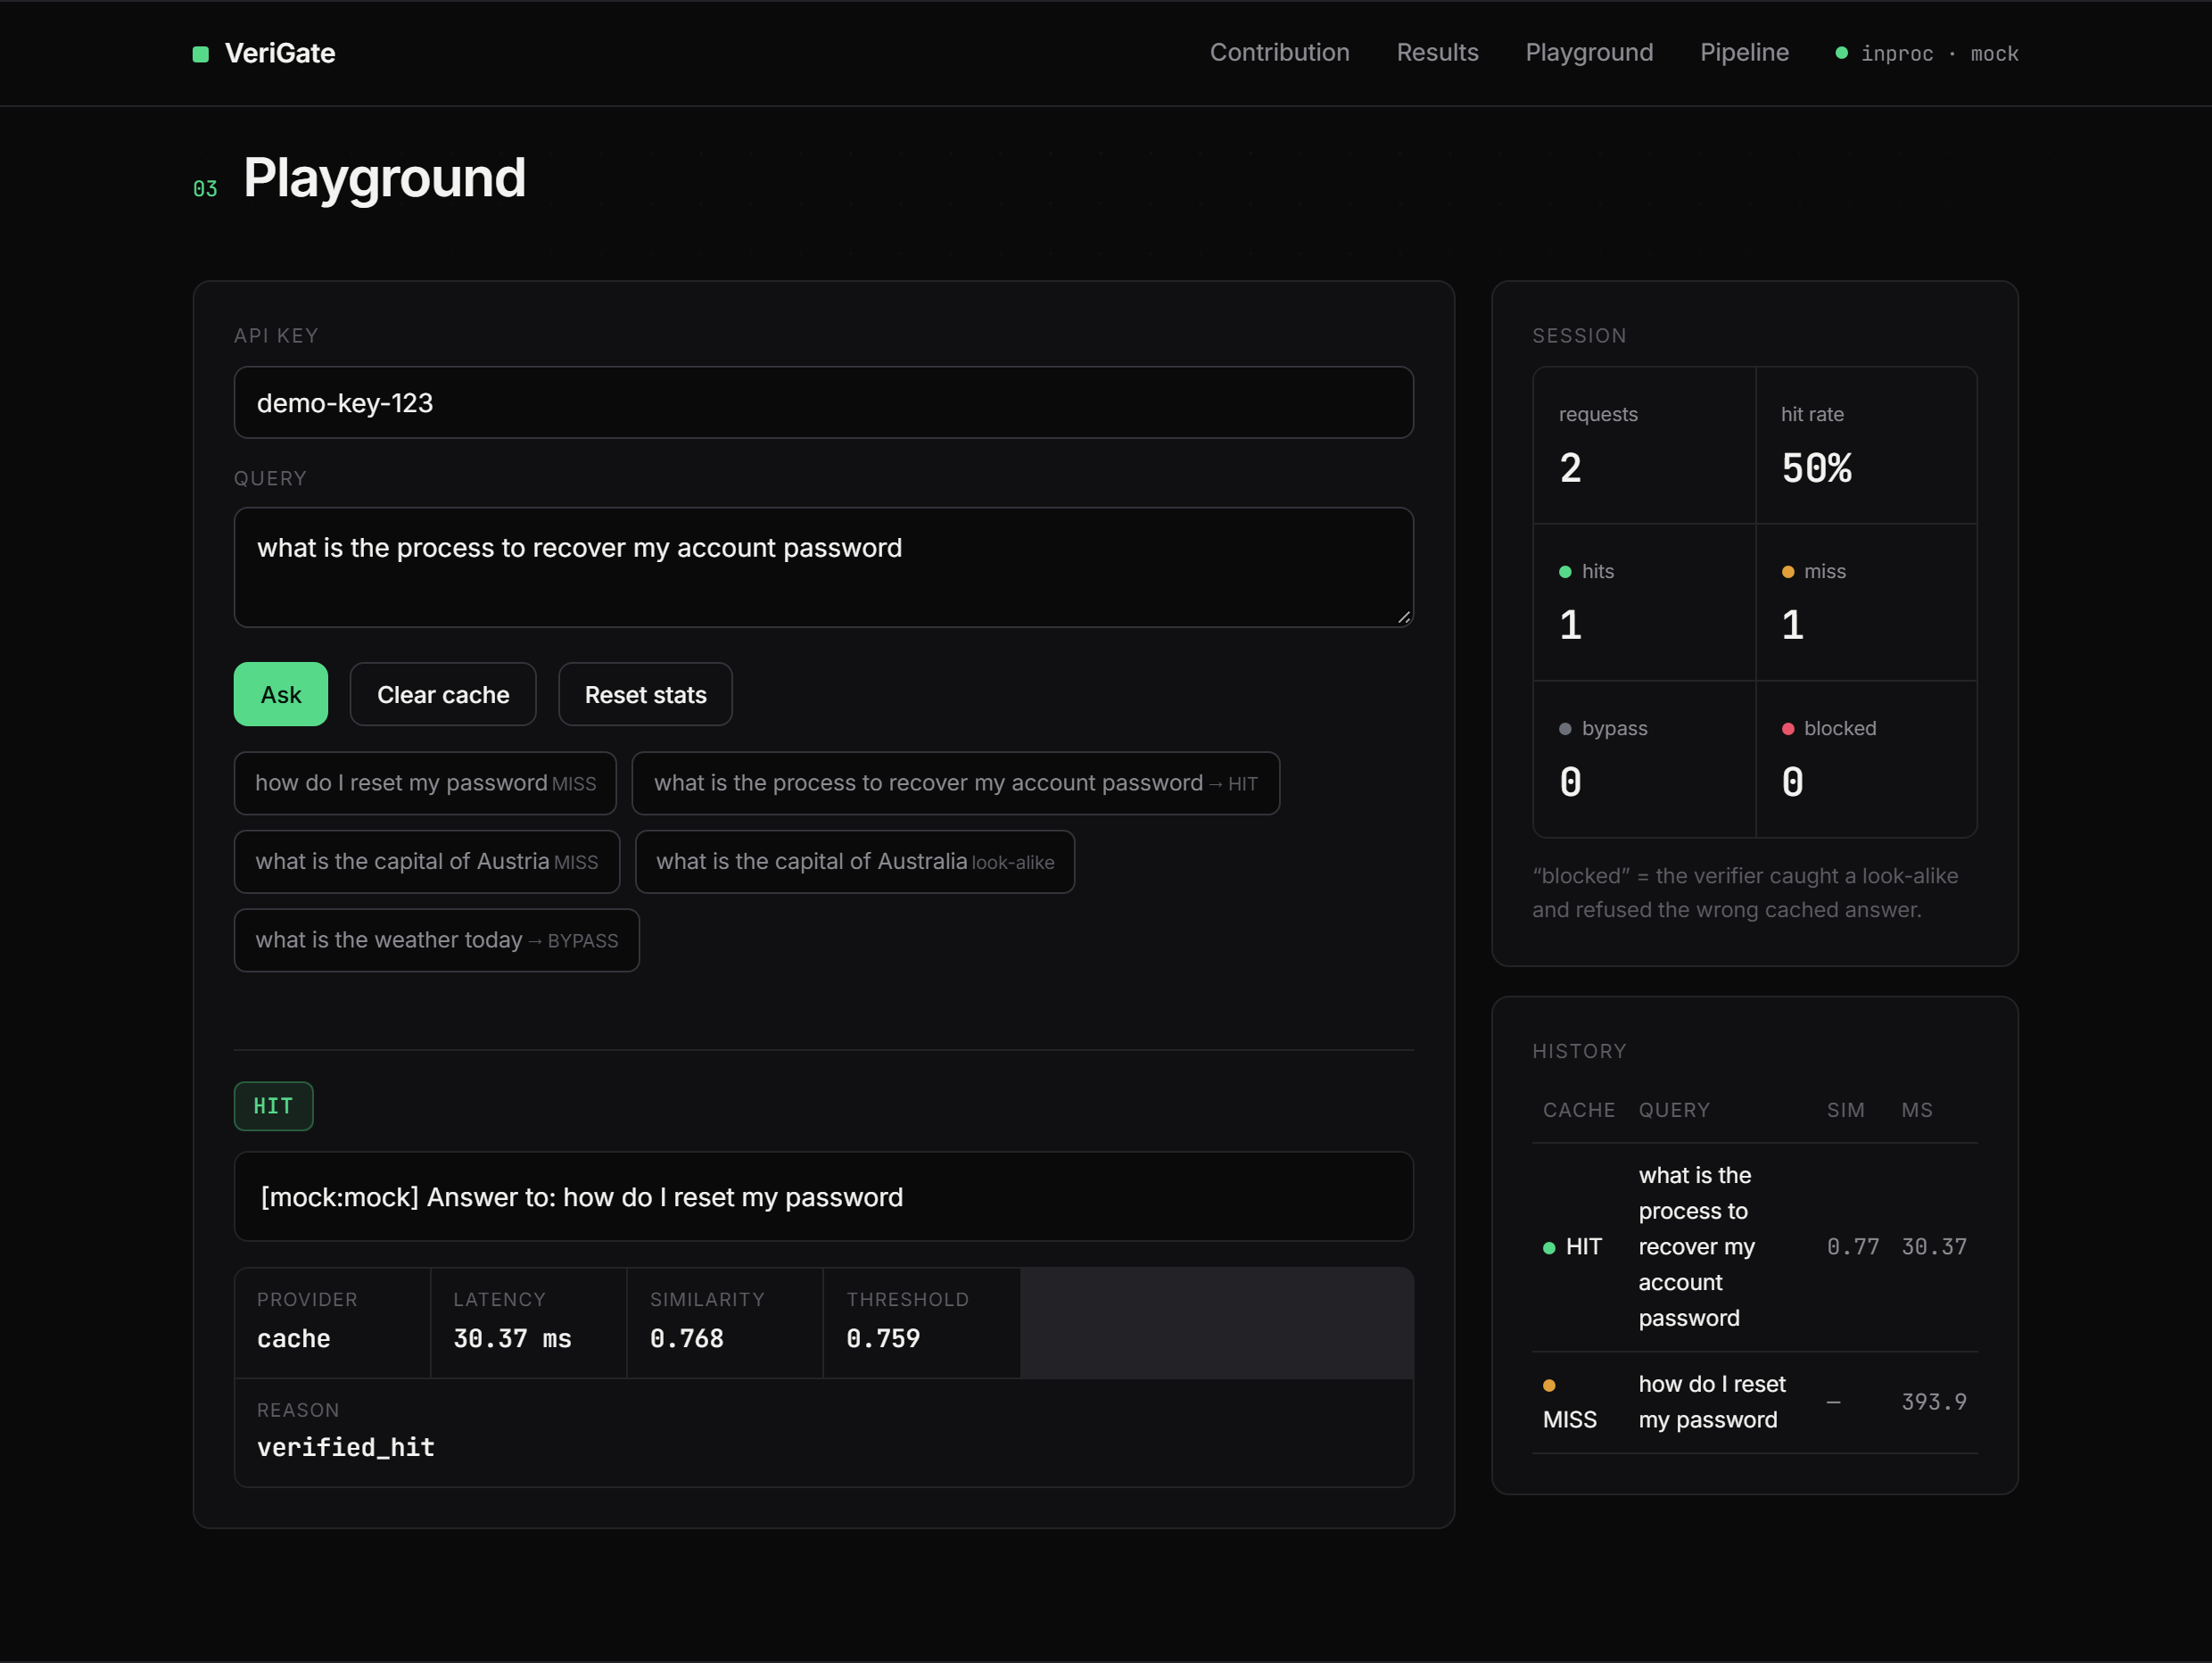
\includegraphics[width=0.90\textwidth]{ui_hit.png}
    \caption{A reworded query (``what is the process to recover my account password'') served as a HIT from a prior ``how do I reset my password'' --- matched by meaning, in $\sim$30~ms.}
    \label{fig:ui_hit}
\end{figure}

\begin{figure}[H]
    \centering
    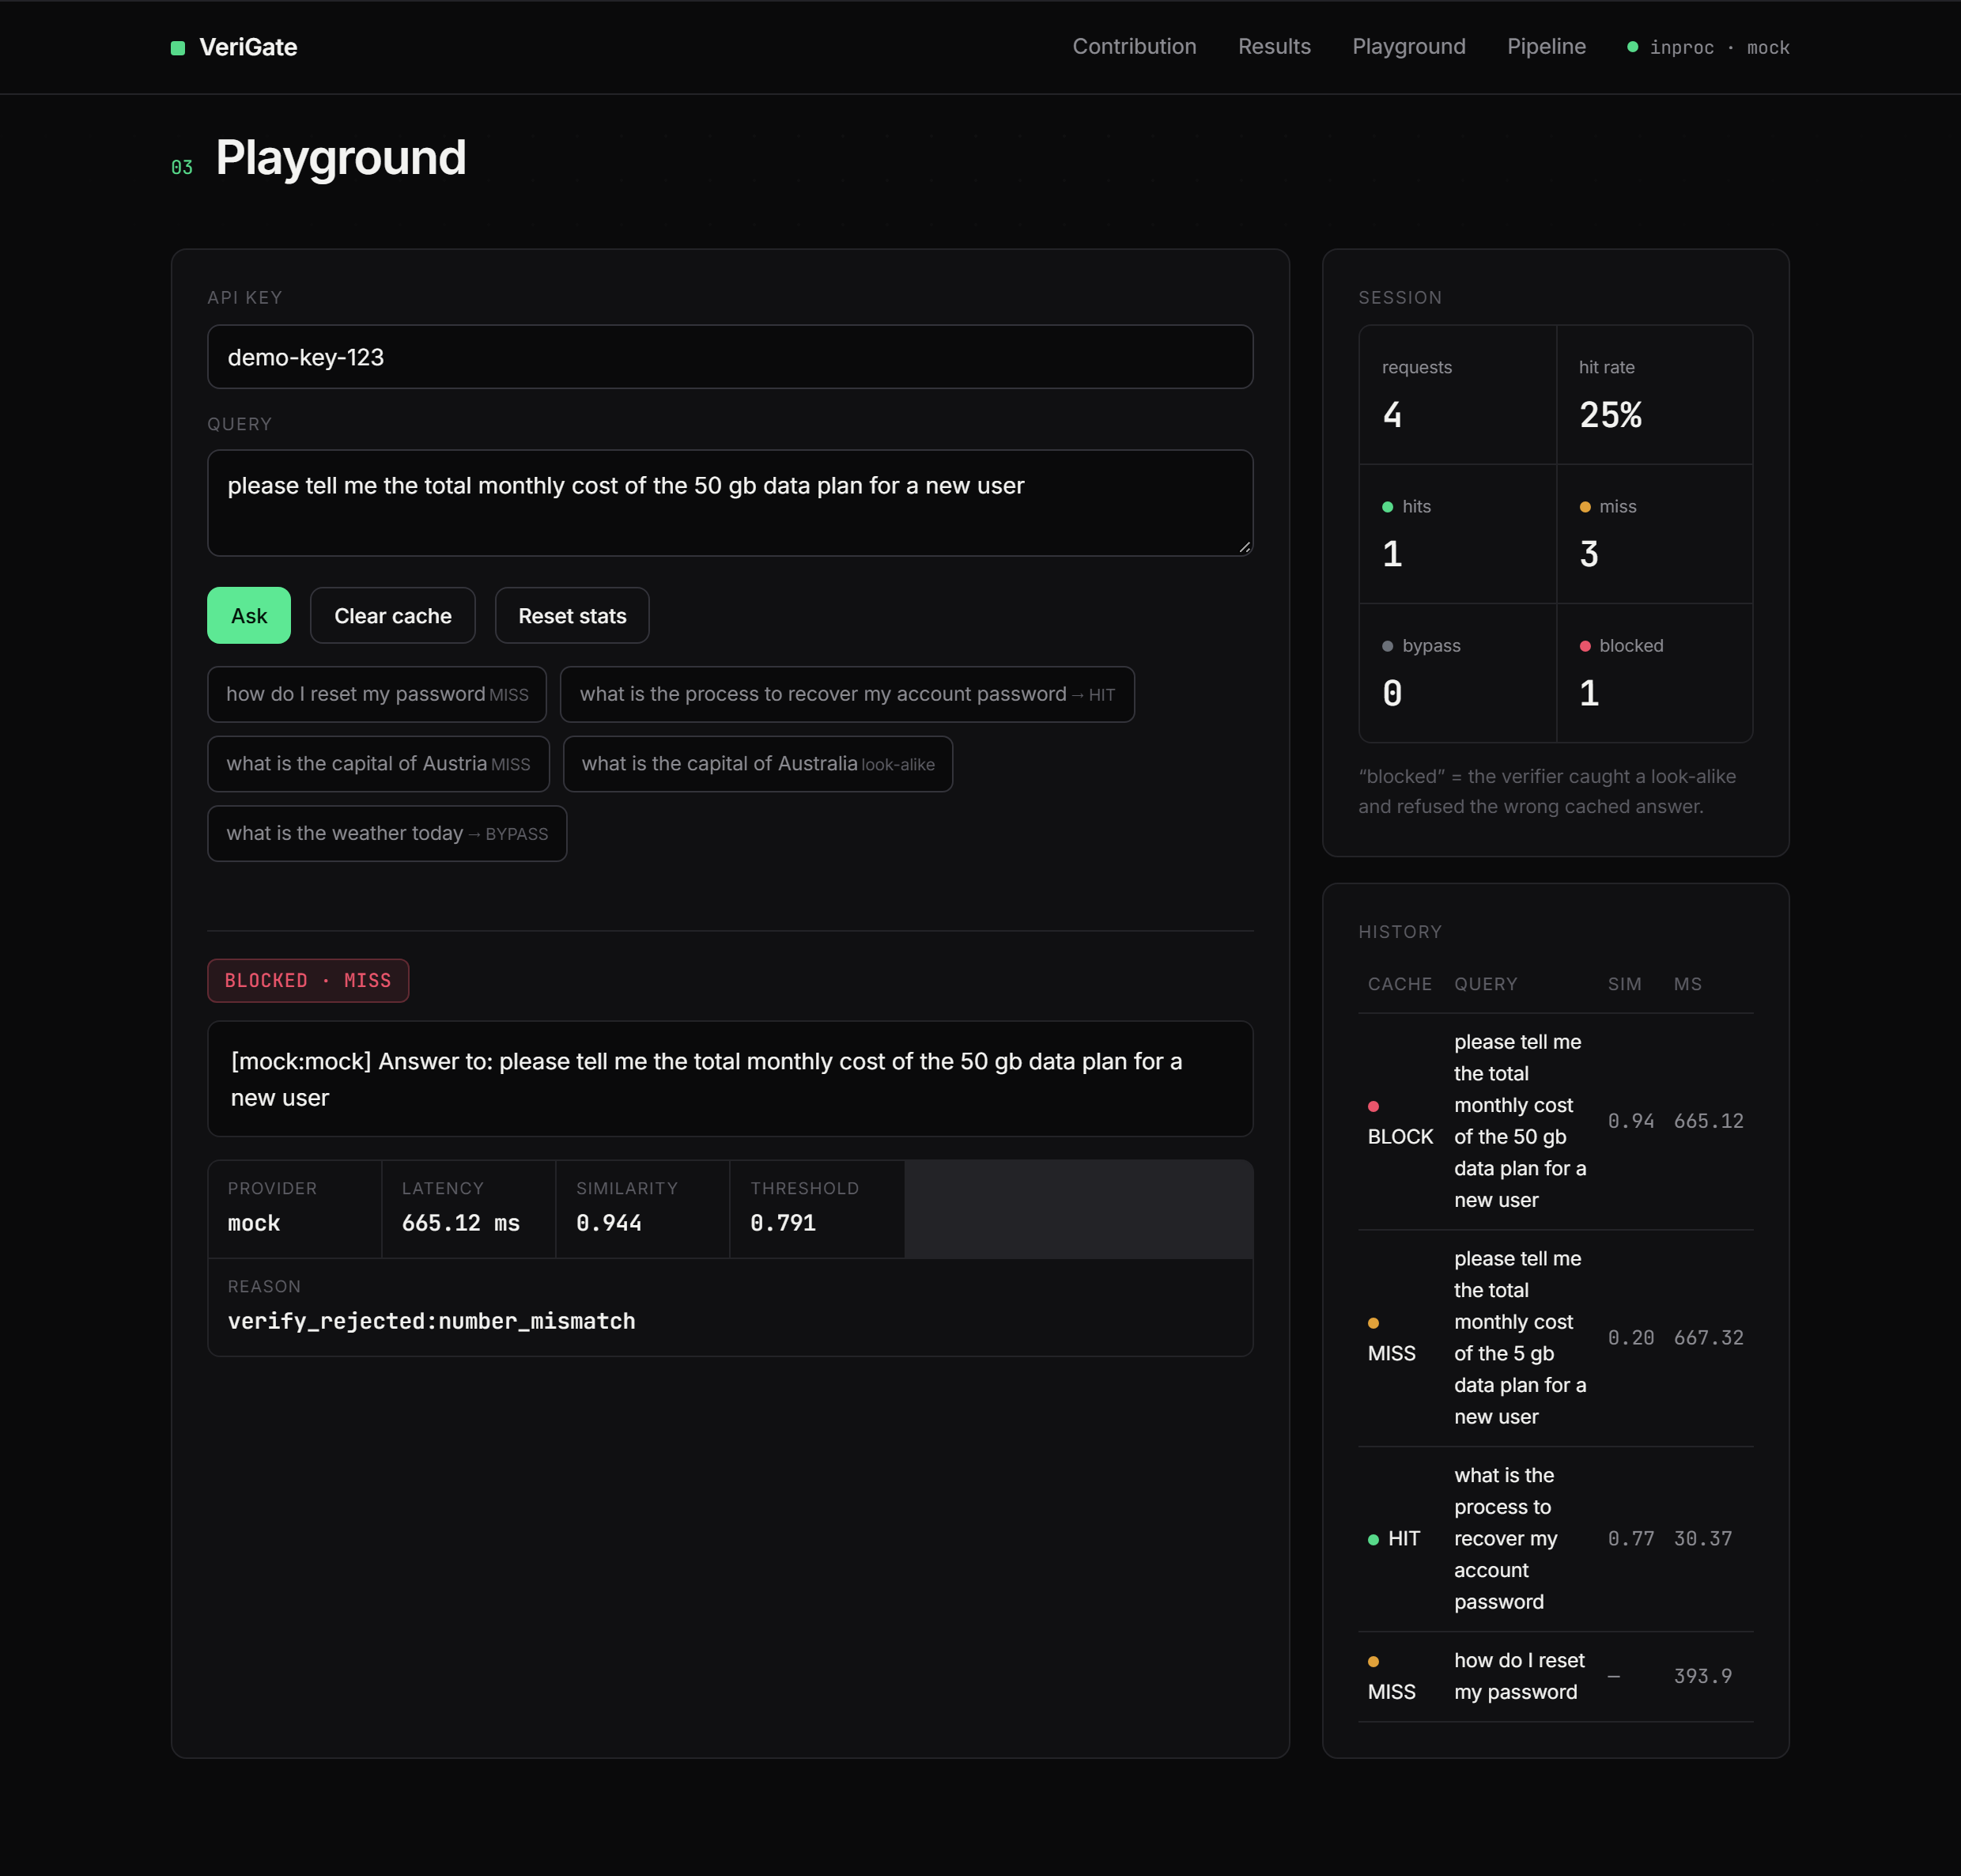
\includegraphics[width=0.90\textwidth]{ui_blocked.png}
    \caption{The self-verifier in action. The ``50 gb'' query is similar (0.944) to a cached ``5 gb'' query --- \emph{above} the adaptive threshold (0.791) --- yet is BLOCKED with reason \texttt{verify\_rejected:number\_mismatch}. This is precisely the false hit a fixed-threshold cache would serve, and precisely what VeriGate prevents.}
    \label{fig:ui_blocked}
\end{figure}

\section{Summary of Results}
VeriGate reduces the false-hit rate from 46.7\% to 0.0\% (100\% precision) at a structural-verification cost of $\sim$0.03~ms; a vectorised index brings the cache-hit path to $\sim$10~ms ($\sim$78$\times$ faster than an LLM call) and keeps lookup sub-millisecond as the cache grows; the cost-aware cascade cuts LLM spend $\sim$47\% with no quality loss on hard queries; and the system is verified secure (tenant isolation), reliable (failover, breaker), observable (Grafana), and live (real Gemini). Collectively these results substantiate every objective of Section~1.4.

        \chapter{Conclusion}
        \section{Conclusion}
The literature survey of Chapter~2 identified a clear gap: semantic caches for LLMs deliver real cost and latency savings but trust a single fixed similarity threshold and never verify a candidate hit, making them unsafe in precisely the look-alike cases --- differing by a number, a negation, or a named entity --- that matter most. In this project we designed, implemented, and evaluated \textbf{VeriGate}, a production-grade LLM Gateway whose core novel contribution is an \textbf{adaptive, self-verifying semantic cache} that closes this gap by separating the \emph{threshold} decision from the \emph{equivalence} decision: an adaptive threshold proposes a candidate, and a cheap-first two-tier verifier disposes of false hits before any answer is served.

The central result is decisive. On a controlled benchmark of hard negatives, VeriGate reduces the false-hit rate from the fixed-threshold baseline's \textbf{46.7\%} to \textbf{0.0\%} (100\% precision), and the ablation by failure mode shows exactly why: the structural verifier eliminates number-, entity-, and negation-swap collisions, while the adaptive threshold clears related-topic ones. Critically, this safety is essentially free --- Tier-1 verification costs only \textbf{$\sim$0.03~ms} on the hit path. A vectorised index reduces the cache-hit path to \textbf{$\sim$10~ms} ($\sim$78$\times$ faster than an 800~ms LLM call) and keeps lookup sub-millisecond as the cache scales, and the analysis of the optional Tier-2 NLI verifier yields a genuine research insight: NLI attains maximal correctness but at a recall cost and is largely \emph{redundant} once the adaptive threshold is enabled, so it is best offered as an opt-in ``max-correctness mode'' rather than a default.

A second contribution, the \textbf{cost-aware model cascade}, complements the cache by cutting LLM spend by \textbf{$\sim$47\%} with no quality loss on hard queries, beating random routing at every operating point. Around these two contributions, VeriGate is engineered as a deployable system: per-tenant cache isolation (closing the defining security risk of a semantic cache, with a regression test guarding it), per-key spend budgets that leave cache hits free, a provider circuit breaker and mock failover, Prometheus/Grafana observability, an interactive operator dashboard, and Docker packaging verified end-to-end. The whole thesis was demonstrated live against real Gemini, where a 23-second paid call became a 22~ms free cache hit --- even for a reworded question. More broadly, the project shows that in a caching system for high-stakes outputs, \emph{verifying a match before trusting it} is not overhead but the feature itself.

\section{Limitations of the Current System}
Despite the strong results, several limitations bound the current system and should be stated honestly:
\begin{enumerate}
    \item \textbf{Benchmark scale.} The evaluation uses a compact, hand-curated benchmark that isolates the mechanism. The \emph{relative} improvement over the baseline is the result; the \emph{absolute} hit-rate and false-hit numbers are dataset-dependent and would shift on a large natural query log.
    \item \textbf{Hand-tuned decision logic.} The adaptive-threshold coefficient, the complexity score, and the volatility rules are transparent but heuristic rather than learned, and were tuned on a small validation set.
    \item \textbf{Tier-1 verifier coverage.} The structural verifier covers numbers, negation, and named entities; subtler semantic distinctions rely on the more expensive Tier-2 NLI stage, which is off by default.
    \item \textbf{Unbounded cache growth.} A per-entry TTL exists, but a maximum-size cap with LRU/LFU eviction is not yet implemented, so memory is bounded only by TTL.
    \item \textbf{Operational surface.} \texttt{/metrics} is public in the demo build, and TLS, security headers, and dependency scanning are deployment-time concerns documented but not enforced in-app.
\end{enumerate}

\section{Future Scope}
The modular design admits several extensions, grouped by horizon:
\begin{itemize}
    \item \textbf{Near-term --- learned threshold and router.} Replace the heuristic adaptive-threshold coefficient and complexity score with lightweight classifiers trained on a validation split, in the style of learned LLM routing \cite{ong2024routellm}, and gate Tier-2 NLI to borderline similarities only with a per-request NLI budget.
    \item \textbf{Near-term --- cache eviction.} Add a maximum-size cap with LRU/LFU eviction and memory monitoring to bound growth independently of TTL.
    \item \textbf{Medium-term --- large-scale evaluation.} Re-run the ablation on a public paraphrase corpus and a real query log at the million-vector scale, tuning the adaptive weights on a held-out split and reporting sensitivity.
    \item \textbf{Medium-term --- distributed scale.} Harden the RediSearch/HNSW backend for multi-replica deployments sharing one cache, and tune HNSW parameters at the target corpus size \cite{malkov2018hnsw}.
    \item \textbf{Long-term --- richer verification and safety.} Extend the verifier with unit-aware and temporal reasoning, add optional prompt-injection and output-moderation middleware, and encrypt cached content at rest with PII-aware do-not-cache classification.
    \item \textbf{Long-term --- productionisation.} Lock down \texttt{/metrics}, integrate a host secret store, add TLS/security headers/CORS and CI dependency scanning, and publish a public deployment as a reference service.
\end{itemize}


        \bibliography{report}
	\bibliographystyle{plain}

\end{document}
